%%\PassOptionsToPackage{english}{babel}
\documentclass[pfe ,titlesmallcaps]{isipfe}
\usepackage[english]{babel}
\addto\captionsenglish{% Replace "english" with the language you use
  \renewcommand{\contentsname}%
    {Table of contents}%
}
\usepackage[table,xcdraw]{xcolor}
\usepackage{nth}
\usepackage[light]{CormorantGaramond}
\usepackage[T1]{fontenc}
\usepackage{lettrine}
\usepackage{kpfonts}
%%\usepackage[T1]{fontenc}
\usepackage[utf8]{inputenc}
\graphicspath{{./Figures/}}
\usepackage{hyperref}
\usepackage{array}
\usepackage{multirow}
\usepackage{acro}
\usepackage{listings}
\usepackage{algorithm}
\usepackage{enumitem}
\usepackage{algorithmic}
\usepackage{wrapfig}
\usepackage{float}
\usepackage{tcolorbox}
\usepackage[]{multibib}
\newcites{A}{Webography}
\usepackage{notoccite}
\usepackage{acronym}
\usepackage{textcomp}
%%\usepackage[frenchb]{babel}
\usepackage{afterpage}

\newcommand\blankpage{%
    \null
    \thispagestyle{empty}%
    \addtocounter{page}{-1}%
    \newpage}

\usepackage{inconsolata}
\usepackage{color}


\definecolor{pblue}{rgb}{0.13,0.13,1}
\definecolor{pgreen}{rgb}{0,0.5,0}
\definecolor{pred}{rgb}{0.9,0,0}
\definecolor{pgrey}{rgb}{0.46,0.45,0.48}


\lstset{language=Java,
  showspaces=false,
  showtabs=false,
  breaklines=true,
  showstringspaces=false,
  breakatwhitespace=true,
  commentstyle=\color{pgreen},
  keywordstyle=\color{pblue},
  stringstyle=\color{pred},
  basicstyle=\ttfamily,
  moredelim=[is][\textcolor{pgrey}]{\%\%}{\%\%},
  moredelim=[il][\textcolor{pgrey}]{\$\$}  
}



 
\begin{document}  

\frontmatter

\title{Titre du projet}
\author{Safoine BENHMIDA}

%%% YOU MUST update information of this page
\thispagestyle{empty}%
\hspace{-1cm}
\begin{minipage}[l]{0.2\columnwidth}

\includegraphics[width=1.1\columnwidth]{LogoISI}\\
\end{minipage}
\hfill
\begin{minipage}[l]{0.6\columnwidth}
\centering
\footnotesize
\textbf{\textsc{Tunisian Republic}}\\
\textbf{\textsc{Ministry of Higher Education\\
and Scientific Research}}\\
\textbf{\textsc{University of Tunis El Manar}}\\
\textbf{\textsc{Higher Institute of Computer Science}}
\end{minipage}
\hfill
\begin{minipage}[l]{0.2\columnwidth}

\includegraphics[width=0.7\columnwidth]{logoutm}\\
\end{minipage}
\begin{center}
    
\end{center}
\begin{center}
{\large{\textbf{\textsc{Bachelor's Thesis}}}}\\
{\textbf{Presented in order to obtain the}}\\
{\textbf{Bachelor's Degree in Computer Science}}\\
{\textbf{Mention: Computer Science}}\\
{Specialty : Computer Science}
\end{center}
\vskip1cm%
\begin{center}
\textrm{By:}\\
{\large\textbf{Safoine BEN HMIDA - Mehdi CHOURA}}\\
%%{\large\textbf{Mehdi CHOURA}}\\
\vskip1cm
%%{\huge\textbf{Semantic Annotation for the “on demand graphical representation” of unstructured data }}\\
\begin{minipage}[l]{1\columnwidth}
        \begin{tcolorbox}[colframe=blue,colback=white,boxrule=2pt,arc=10pt,height=30mm]
         \vskip1mm
            \centering
        {\LARGE\textbf{Semantic Annotation for the “On demand graphical representation” of unstructured data}} 
        \end{tcolorbox}
    \end{minipage}
\end{center}
\vskip1cm%
\begin{center}
\begin{minipage}[c]{0.11\columnwidth}
\end{minipage}
\hfill
\begin{minipage}[c]{0.29\columnwidth}
Laboratory supervisor:\\
Academic supervisor:
\end{minipage}
\hfill
\begin{minipage}[c]{0.47\columnwidth}
\textbf{Ramzi GUETARI}\\
\textbf{Nour El Houda BEN CHAABENE}
\end{minipage}
\hfill
%%\begin{minipage}[c]{0.29\columnwidth}
%%Maître assistant\\
%%Maître assistant
%%\end{minipage}
\end{center}
\vskip1cm
\begin{center}
{Realized within LIMTIC Laboratory}\\
\vskip1cm

\includegraphics[width=0.4\columnwidth=2cm]{LIMTIC}
%%
\includegraphics[width=0.2\columnwidth,height=2cm]{riadiup}\\
\end{center}
\vskip1cm%
\begin{center}
{\textrm{Academic year : 2016-2017}}\\
\end{center}
\vfill
\newpage
\chapter*{Dedications}

\begin{center}
I want to dedicate this humble work to: \\
\end{center}
\begin{center}
My parents \textbf{Slah Eddine} and \textbf{Hamida} for all the pain they have been through and all the sacrifices they made in order for me to reach this level and for me to be what I am today.\\
\end{center}
\begin{center}
To my siblings, Rihab and Ghofrane and Hassen for their patience, continuous support and care.
\end{center}
\begin{center}
To all the members of my family especially Oussama and my dearest friends: Bacem, Amine, Ghaith, Mokhtar, Malek,  Meriem and all the ones I didn’t mention for the best times and laughs we had and sticking by my side the time I needed. \\
\end{center}
\begin{center}
For all those I love and all those who love me.
To all who helped that I forgot to mention.
\end{center}


\begin{flushright}
With Love,

Safoine Benhmida.
\end{flushright}
\chapter*{Dedications}

\begin{center}
I want to dedicate this work:
\end{center}
\begin{center}
To my father Mohamed for being my guardian during my educational career. To my mother Fattouma who support and encourage  me to believe in myself. 
\end{center}
\begin{center}
To my brother Khalil and my sister Asma who show always the best path to follow. 
\end{center}
\begin{center}
To my friends Ghaith, Amine, Bacem for their help and advice.
\end{center}
\begin{center}
Finally, I would also like to thank everyone who has been involved in this work that I forgot to mention.
\end{center}

\begin{flushright}
With love,

Mehdi CHOURA.
\end{flushright}
\chapter*{Acknowledgements}

\begin{center}
\emph{We would first like to thank and express my very profound gratitude to our academic advisor, Mrs. \textbf{Nour EL Houda BEN CHAABENE} for the huge effort and sacrifice she gave the entire time and also for believing in our capacities and her patience, motivation, and immense knowledge. Her guidance helped us in all the time of research and writing of this thesis.}\\
\end{center}
\begin{center}
\emph{Our academic Professor, Mr. \textbf{Ramzi GUETARI}, for his big support and generosity and his continuous welcome in his office that was always open whenever we ran into a trouble spot or had a question about our research, and steering us in the right direction whenever we needed it.}\\
\end{center}
\begin{center}
\emph{We would also like to show our gratitude to the Mrs. \textbf{Maha MALLEK} for sharing her pearls of wisdom with us during the course of this research, and her help throughout the writing of the thesis.} \\
\end{center}
\begin{center}
\emph{We also thank our fellow labmates in for the stimulating discussions and for all the fun we have had in the last couple of months.}\\
\end{center}
\begin{center}
\emph{Also  anyone who contributed to this work for the support, even spiritually especially the last couple of weeks.}\\
\end{center}

\begin{flushright}
With Gratitude

Safoine.

Mehdi.
\end{flushright}


\setcounter{secnumdepth}{3}
\setcounter{tocdepth}{3}
\tableofcontents

\listoffigures
\listoftables
\lstlistoflistings
\chapter*{Acronyms}
\markboth{}{}
%%AJAX ............ \\
\begin{acronym}
  \acro{AJAX}{Asynchronous JavaScript And XML}
  \acro{API}{Application Programming Interface}
  \acro{CERN}{European Organization for Nuclear Research}
  \acro{CSS}{Cascading Style Sheets}
  \acro{DL}{Description Language}
  \acro{DOM}{Document Object Model}
  \acro{DTD}{Document Type Definition}
  \acro{GPL}{GNU General Public License}
  \acro{GUI}{Graphical User Interface}
  \acro{HTML}{HyperText Markup Language}
  \acro{IDE}{Integrated Development Environment}
  \acro{ISI}{HIGHER INSTITUTE OF Computer Science}
  \acro{JS}{JavaScript}
  \acro{JSP}{Java Server Page}
  \acro{NER}{Named Entity Recognition}
  \acro{NLP}{Natural Language Processing}
  \acro{OWL}{Ontology Web Language}
  \acro{RDF}{Resource Description Framework}
  \acro{RDFS}{Resource Description Framework Schema}
  \acro{RSS}{Really Simple Syndication}
  \acro{SGML}{Standard Generalized Mark-up Language}
  \acro{SPARQL}{SPARQL Protocol and RDF Query Language}
  \acro{URI}{Uniform Resource Identifier}
  \acro{URL}{Uniform Resource Locator}
  \acro{WWW}{World Wide Web}
  \acro{W3C}{World Wide Web Consortium}
  \acro{XML}{eXtensible  Markup Language}
\end{acronym}

\afterpage{\blankpage}


\mainmatter
%%%%% Introduction
\addcontentsline{toc}{chapter}{Background and motivation}
\chapter*{Background and motivation}
\label{Intro}
 
\lettrine[lines=3,loversize=0.5]{T}{}he Web is a major technology in 2\nth{1} century. Its birth came after Internet and hypertext combination. Over the past decades, the use of the Web have changed a lot - it has influenced our social and commercial activities. In the beginning, Web was static - it transmits information using static HTML (Hypertext Markup Language) documents. After few years, new Web languages have been created like CSS (Cascading Style Sheets), JavaScript and much more in order to improve the performance of the Web .
With the appearance of social media, e.g. Facebook, Twitter, Youtube, that have been invading the Web and have eased the set of personal relations. The use of internet has continued to rise and become a daily routine for most of people.
At the beginning of the 2000's, Web have ameliorate the work of search engines by organizing the big amount of data considering their semantic by annotating documents .\\
New other languages were created like RDF (Resource Description Framework), RDFS (Resource Description Framework Schema)
, SPARQL (SPARQL Protocol and RDF Query Language) that form the base and fundamental of semantic Web.\\



The semantic Web aims to develop a smart Web that holds resources which can be understood by both human and computers. It basically uses annotations and Ontologies. The word “Ontology” is used with different senses in different communities. The most radical difference is perhaps between the philosophical sense, which has of course a well-established tradition, and the computational sense, which emerged in the recent years in the knowledge engineering community, starting from an early informal definition of (computational) Ontologies as \textit{"explicit specifications of conceptualizations"}. Ontology definition in philosophy is \textit{"The study of being as a being"} but in computer science field is a model to represent the meaning of the knowledge of a domain. To represent an Ontology, W3C created a standard language OWL (Ontology Web Language), built on the RDF data model. It adds the ability to define classes in more complex connectors corresponding to the description logic. Ontology is therefore used to reason about the objects of a certain domain concerned.
The conception of an Ontology includes both building of a model of knowledge representation and the enrichment of that model (
attachment to the elements components the schema of instances coming from the resources of the cooperating systems). An ontology corresponds to a common controlled, organized, and shared vocabulary and to the explicit formalization of the relations created between the different terms of the vocabulary.\\

The works already carried out within the Semantic Web is limited to the processing of textual information. To date, there is no way to synthesize information in the form of dynamic graphics generated on demand and which conform to the data that accompanies them. Therefore, it exists the variable data that can change, so we need to generate a graphic when the user needs it. The semantic Web can not provide an semantic annotations for the on demand graphical representation of variable data in Web documents. \\ 

As an example, let us consider an election period, the French presidential election of 2017 for instance. People would like to have an idea about the trends and the scores that could be obtained by each candidate. A simple search on the Web may lead to a huge amount of textual data that could be impossible to manage as is. However, the best way to represent trends in general is a graphical representation.
At the present time, graphical representations of such trends are given by simple static images. However these images may be too old and do not represent the real trends. The graphic synthesis of the textual information is a way to facilitate the understanding and the manipulation of the data. Every dynamic or variable phenomenon may be represented graphically. The variable may be quantitative or qualitative. It may also be a stochastic variable. The graphical representation of a variable data must be consistent with the data source in order to be credible and effectual.

Our objective is to implement an approach that allows to automatically analyze documents in order to  extract context and relations and to provide a semantic annotation that means to enable the graphical representation on demand. \\


This report comports four chapters. In the first one, we present the evolution of Web and the technologies. In the second chapter, we discuss the birth of the semantic Web, its architecture and its basic bricks (technologies and languages). In the third chapter, we focus on the usefulness of graphical information synthesis and we illustrate theoretically our general process of graphical representation on demand. In the last chapter, we demonstrate the process's implementation. \\






%%%%% Chapter one
\chapter{The Web's first steps}
\label{chap_one}

\section*{Introduction}
In October 1967, a plan for a computer network, called by ARPANET (Advanced Research Projects Agency Network)\cite{history}, was presented. Three years later, the first four-computer network was up and running, making it the first step towards today's network. Later in 1982, ARPANET had officially launched the TCP/IP - the Internet, as we know it, had arrived, which finally led to the birth of the World Wide Web in the 1990s. 
\newpage


\section{Web's first generation}
\label{sec_web}
 
\subsection{History}
\label{subsec_history}
The ideas behind the World-Wide Web were formulated at CERN (European Organization for Nuclear Research) in 1989, leading to a proposal submitted in November 1990 by Tim Berners-Lee and Robert Cailliau for a “Universal hypertext system” [1]. In the four years since the original proposal, the growth of the World Wide Web had been phenomenal. It was mainly used for research applications thus, it quickly expanded until it reached people’s homes.
The World Wide Web is designed around hypertext documents that are simple in which words, phrases, or images act as links to other documents through Client-Server architecture, where the documents are stored in the server’s hard drive and can be consulted by clients from the same network through the HTTP. These documents are classified as a set of HTML pages.
In July 1994, CERN began to overturn the Web project to a new group called the W3 organization, which is now known as the W3C (World Wide Web Consortium) that was founded by Tim Berners-Lee  \cite{hist}.

In 1995, 18 million American homes were already online and Microsoft had just launched the first version of Internet Explorer, the rival of Netscape. Later that year, the first search engine “AltaVista” was introduced. It was the first and most important search engine amongst all others because it led the way for Google, the best search engine by far, to be launched in 1998. It uses automated programs called spiders like most other engines do and has a large index of keywords. It also ranks each Web page after determining their relevancy.


\subsection{Web's first technologies}

Shortly after the birth of the Web, several technologies were built. They led the way for many other languages and features to come in the next few years.  


\subsubsection{SGML}
\label{subsubsec_sgml}
The SGML (Standard Generalized Markup Language) is a standard of ISO (International Organization for Standardization) under the ISO 8879 standard. It is a standardized markup language for describing the structure and formatting of a computer document. Sections of the document are set off by embedded tags. The tags and the relationships among the groups they represent are described in a DTD (Document Type Definition). The tags do not directly specify what the display of the document will look like, so different applications can display the information differently. 

\subsubsection{DTD}
\label{subsubsec_dtd}

DTD  (Document Type Definition) is a set of markup declarations that can be used to define a document type for SGML documents. Since XML is a subset of SGML, DTD can also be used to define a document type for XML documents. If an SGML or XML document is said to be valid against a DTD document type, all elements, attributes and entities in the document must meet their declared formats described in the DTD document type. The DTD can be written inside or outside the markup language document as DTD file. Here is a simple example of a DTD document type (Listing \ref{dtdfile}), where the root element is a candidate which is defined with the sub elements: name, age, occupation and residence.\\  

\begin{lstlisting}[captionpos=b, caption=An example of a DTD file, label={dtdfile},
basicstyle=\footnotesize,frame=none]
<!ELEMENT candidate (name,age,occupation,residence)>
<!ELEMENT name (#PCDATA)>
<!ELEMENT age (#PCDATA)>
<!ELEMENT occupation (#PCDATA)>
<!ELEMENT residence (#PCDATA)>
]>     
\end{lstlisting}


\subsubsection{HTML}
\label{subsubsec_html}


HTML (Hypertext Markup Language) is a simplified derivative of SGML. It is also defined with a DTD and must meet all the markup declarations located inside the DTD in order to be valid.  Each HTML document is divided into a heading section and a main body. HTML also distinguishes headers, lists, tables, forms, etc. It is also possible to insert images or animations at specific positions in a document. 
Originally, HTML was primarily designed as a language for semantically-describing scientific documents. Its general design, however, has enabled it to be adapted over the subsequent years to describe a number of other types of documents and applications. In October 2014, HTML5 [3] was standardized by the W3C. The current version of HTML now is HTML 5.1 [4] that was recommended by the W3C in November 2016. 


\subsubsection{URL}
\label{subsubsec_url}
The final and most important keys to the World Wide Web are the URLs that allow the hypertext documents to point to other documents located anywhere on the Web. 
A URL consists of three major components: 
%%<protocol> :// <node> / <resource name> \\
\begin{lstlisting}[captionpos=b, caption=URL components, label=url, belowskip=1em, aboveskip=2em,frame=single,]
	"  <protocol> :// <node> / <resource name(path)>  "
\end{lstlisting}

 The first component specifies the protocol to be used to access the document, e.g. HTTP, FTP, etc. The second component, called the node, specifies the hostname and the file path on the network from which the document is to be obtained, and the third component specifies the location of the document on the remote machine.


\subsection{Limitations of the first generation of the Web}

The Web is limited to the use of static HTML documents, the lack of context and the absence of human interaction. This led to move to a new generation of the Web.  

% Une section
\section{Web's second version}
\label{sec_web2_0}

% Une sous section
\subsection{Preface}
\label{subsec_pres_web_2_0}

The second generation of the Web \cite{web2030} had introduced  to a diversity of new applications and services of the Web such as social networking (Facebook, Twitter, ...), blogging, wikis, photo and video sharing (Youtube, Flickr, ...), tagging, etc. What these new applications had in common was that the user had become the source of information on the Web. These new dynamic Web apps are distinguished by some features : 

 \begin{itemize}
 \item \textbf{Folksonomy:} It's the free classification of information on the World Wide Web known as social tagging.
 \item \textbf{Rich User Experience:} The social Web uses new technologies presenting dynamic and rich user experience to users. %%Unlike the first generation of the Web  ;
 \item \textbf{User As Contributor :} The user is able to contribute to the content by means of Evaluation, Review and Commenting, etc.
 \end{itemize}
		
\subsection{New technologies and Languages}
\label{subsec_app_tech}
\subsubsection{XML}
XML (Extensible Markup Language) is a formal recommendation from the W3C \cite{xml}, and is similar to HTML for containing markup symbols. An XML document contains elements defined by tags. An element has a beginning and an ending tag. All elements in an XML document are contained in an outermost element known as the root element. This allows XML to support hierarchical structures.  

In order for an XML document to be valid, all elements, attributes and entities in the document must meet their declared formats described in the DTD document type.\\
The listing \ref{dtdfile} above shows the DTD related to the XML document shown in the listing \ref{xmlfile} below.

\begin{lstlisting}[captionpos=b, caption=An example of an XML file, label={xmlfile},
basicstyle=\footnotesize,frame=none]
<?xml version="1.0"?>
<candidate>
  <name> Francois Fillon </name >
  <age> 63 </age >
  <occupation> French politician </occupation >
  <residence> Le Mans </residence >
</candidate>
\end{lstlisting}

\subsubsection{XML Schema}
Similar to DTD, XML Schema \cite{xmlshema} is also a language for expressing constraints about XML documents. It is usually named XML Schema Definition or simply XSD file. Unlike DTD documents, XML Schema uses an XML-based syntax, whereas DTDs have a unique syntax. It defines datatypes for elements and attributes while DTDs do not. It also defines the number and order of child elements, while DTDs do not. And most importantly XML schema is extensible, while DTDs are not.\\
The listing \ref{xmlfshema} below, shows the content of an XSD file that defines and describes the XML document shown in the listing above \ref{xmlfile}. 

\begin{lstlisting}[captionpos=b, caption=An example of a XML Schema file, label={xmlfshema},
basicstyle=\footnotesize,frame=none]
<?xml version="1.0"?>
<xs:schema xmlns:xs="http://www.w3.org/2001/XMLSchema">
  <xs:element name="Candidate">
    <xs:complexType>
      <xs:sequence>
        <xs:element type="xs:string" name="name"/>
        <xs:element type="xs:string" name="age"/>
        <xs:element type="xs:string" name="occupation"/>
        <xs:element type="xs:string" name="residence"/>
      </xs:sequence>
    </xs:complexType>
  </xs:element>
</xs:schema>

\end{lstlisting}

\subsubsection{RSS}

RSS (Really Simple Syndication) \cite{rss} is a Web service that has a main focus of facilitation of browsing for news and updates related to a certain website. The RSS feed is an XML document that is usually used by news, companies' sites, or blogs in order to quickly represent their latest information (e.g. headlines, articles,events, etc.) automatically. RSS feed can be gathered and sorted using a software called RSS Aggregator that checks automatically for new content and immediately converts this new content to a readable format. Browsing websites can be very time-consuming especially with low bandwidth. Thus, with the use of RSS feed, users could save plenty of time.

\subsubsection{DOM}

DOM (DocumentObjectModel) is a neutral interface that allows languages and scripts to have a dynamic access and update of the content, structure and style of XML and HTML documents\cite{dom}. \\
The first level of DOM, published in 1998, is separated in two parts: the HTML and Core. The document is presented as a tree of document's elements like paragraphs, buttons, and list. It allow to parse, add, delete, and modify its elements.  \\ 
The DOM level 2, published in 2000, is build on DOM level 1 and has 6 parts: Core, HTML, Events, Style, View and Traversal and Range. It allows immediately to identify an element or group of elements in a document. Also, it offers a direct access to a particular element in the document using the function getElementById() \cite{dom2}.\\
The Dom level 3, published in 2004, comes with XPath module, keyboard events module and XML documents serialisation interface.\\
The DOM level 4 is currently in development. The Last Call Working Draft was in February 2004. 


\subsubsection{CSS}

CSS (Cascading Style Sheets) is a language that describes the style of an HTML document including the colors, borders, backgrounds ... \\
Using HTML, we can define the structure and the style of a Web page however, the presentation is limited \cite{css} , so it is recommended to separate the structure from the style to ease the maintenance of sites.\\
A CSS rule-set consist of a selector and a declaration block:\\
The selector points to the HTML tags to style.\\ 
The declaration block is surrounded by curly braces and contains declarations of rules separated by semicolons.\\
Each declaration includes a CSS property name and a value, separated by a colon \cite{css2}.\\
In the following example, all <h2> elements will be center-aligned, with a blue text color:

{\tt \small
\centering
\begin{verbatim}
 h2 {
    color: blue;
    text-align: center;
}
\end{verbatim}
}




\subsection{Other Web Technologies}

Many languages and technologies have been introduced to make Web more interactive but they are not W3C recommendations.

\subsubsection{JavaScript}

JavaScript is an oriented object and scripts programming language that specify the behavior of Web pages making it more dynamic and interactive with the user.\\
JavaScript is a client-side language, that means that the script is executed by the browser in the user side. In fact, the browser execute the code embed within <script> HTML tag.


\subsubsection{AJAX}

AJAX (Asynchronous JavaScript And XML) aims to optimise the interactivity and the use of Web applications. AJAX allows Web pages to be updated asynchronously by exchanging data with a Web server behind the scenes. This means that it is possible to update parts of a Web page without reloading the whole page \cite{ajax}.
AJAX is the combination of many languages and technologies as presented in figure \ref{fig_Ajax} :
\begin{itemize}
    \item HTML and CSS to represent the Web page.
     \item DOM to describe the interface and display or use the data.
     \item XMLHTTPRequest to request data from a Web server.
     \item XML to structure recovered files from the server.
     \item JavaScript to exploit the XMLHTTPRequest and DOM.
\end{itemize} 
 %%\newpage 

\begin{figure}[H]
\centering
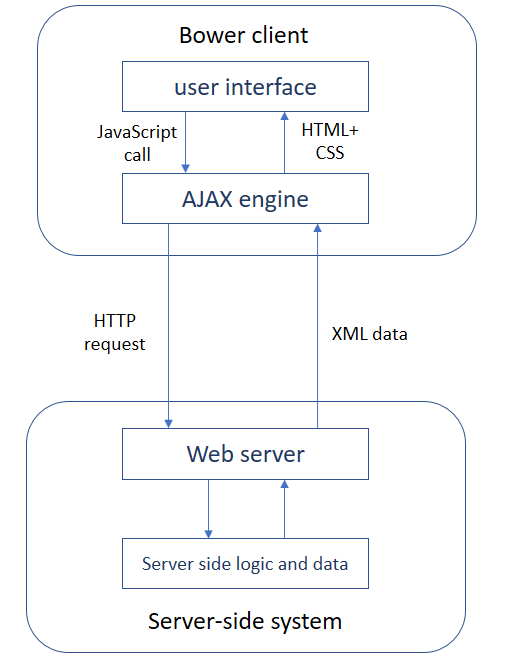
\includegraphics[scale=0.4]{ajax}
\caption{AJAX architecture }
\label{fig_Ajax}
\end{figure}


\subsection{Limitations of social Web }

Although new technologies have evolved within the second generation of the Web, a number of limitations can be identified:

\begin{itemize}
    \item Time and cost consuming: Big projects of social Web application generally take a lot of time to accomplish. 
    \item Short life of information: Once an information on the Internet gets updated, we simply cannot keep track of it so it loses its relevance gradually.  
    \item Lack of semantics: Web applications are still using legacy databases (e.g: Relation databases) without generating and representing knowledge bases.
\end{itemize}


\section{Information search in Web}

\subsection{Search engines}

A search engine is a program that returns a list of Web documents where specific keywords in the query were found \cite{search}.\\
A search engine is a database that is permanently updated by Robots or Spiders that fetch the Web pages, save their contents, and index automatically. There are many popular search engines, e.g. Google, Bing, Yahoo, Ask, etc.


\subsection{Anatomy of search engines}
To provide a pertinent search in the Web, the search engine must have 3 essential parts:
\begin{itemize}
    \item The robot (also known as Spider or Crawler).
    \item The store or the database, that includes the indexer, indexes and complex search algorithms.
    \item The Query or search Interface.
\end{itemize}

The architecture of search engines is shown in the next figure \ref{fig_search_engine}:

\begin{figure}[H]
\centering
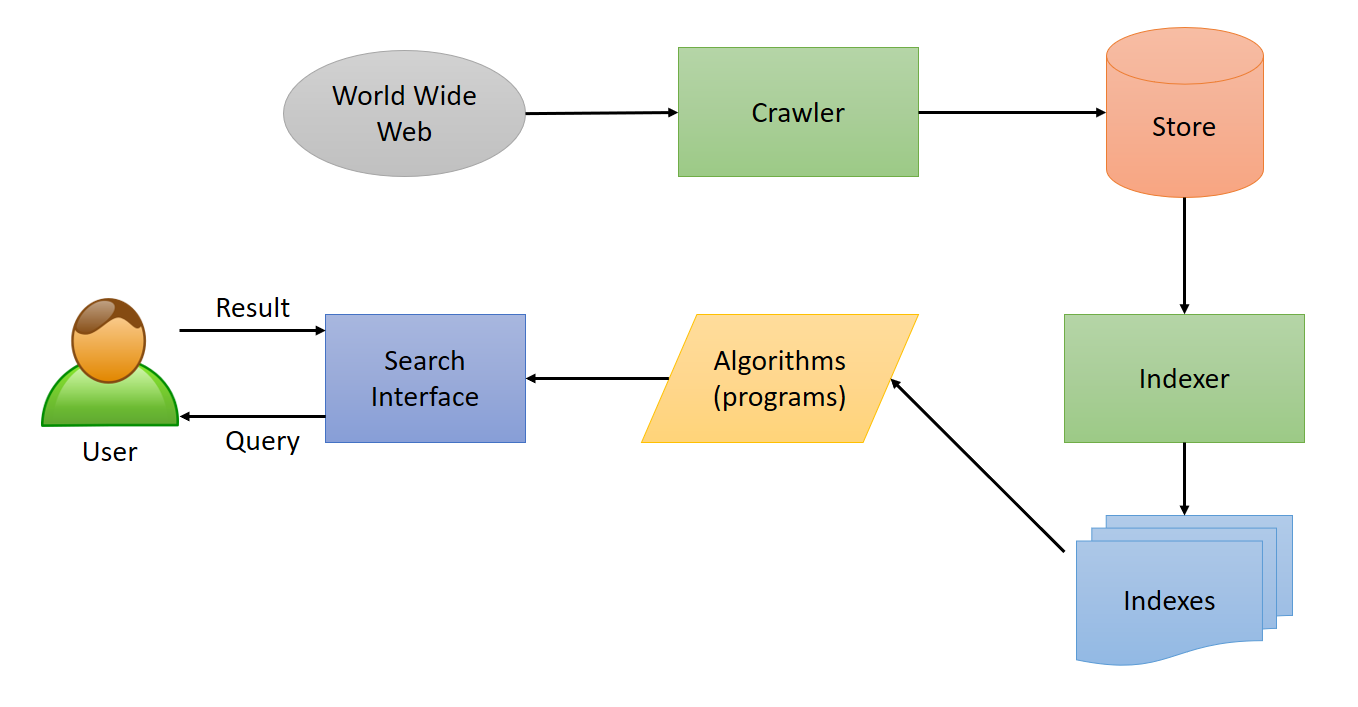
\includegraphics[scale=0.4]{searchengine}
\caption{Search engines architecture }
\label{fig_search_engine}
\end{figure}

\subsubsection{Robot}
Also called Spider or Web-crawler, the robot is the most essential part in the search engine. It collects information from Web documents to be indexed in the database. A Spider can begin almost anywhere because most Web page contains links of other pages. As soon as it sees a link to another page, it goes off and fetches it. \\Alta Vista is an example of a search engine who has many spiders working in parallel\cite{spider}.
\subsubsection{Index}
The Index is where parsed Web pages by the Spider are saved. It contains URLs and the page's title and keywords. When the Robot parse Web pages, it automatically updates the index.\\
There are many ways to index a Web page that distinguishes a search engine from another by results of a keyword query. When the robot fetches the Web pages, it uses different methods to index its content, among the best known:\begin{itemize}
    \item Full-text indexation.
    \item Manual indexation the uses a file edited by person who wants the presence of their Web pages in the database of the search engine. 
    \item Indexation by specific HTML tags (Meta,Title...).
    \item Static indexation which saves the scoring of words in the database.
\end{itemize}
\subsubsection{Query Interface}
The Query interface allows to the user to enter his query using keywords which will then be searched in the index.\\
The interface chooses among the Web pages in the index which satisfy the query and sort them in descending order of relevance, then the user can access to them using a hypertext link. 


\newpage %% a changer si nécessaire 
\section*{Conclusion}

The Web's main purpose was to be designed as a tool to share information across the world. It started with the basics of sharing a document, but has gone on to create tools that are currently known as Web applications, these tools allow us to improve and share our lives (social Web) and much more. The Web is constantly changing and evolving and it will be superseded by something even greater, faster and better. Notably, up on explosion of information amount accessible through the Web, the past versions have encountered drawbacks such as:

%%Today’s World Wide Web has achieved a great evolution. It is widely used all around the world. The simple foundations, on which it is based, has given its strength and global community. Almost every user is able to create and publish hypertext resources in a simple manner. Notably, up on explosion of information amount accessible through the Web, the past versions have encountered drawbacks. The huge amount of content required to be processed in order to find desired facts such as: 

\begin{itemize}
    \setlength{\itemsep}{0cm}
    \setlength{\parskip}{0cm}

    \item Difficulties in finding correct information through simple searching and browsing mechanisms,
    \item Problems of finding facts, which has common correspondents,
    \item Irrelevant results after providing more complex queries in the browsing engines,
    \item Lack of semantics,
    \item Lack of deduction facilities.
\end{itemize}




%Pour faire appel à cette of figure, il suffit d'utiliser le label comme suit:

%La figure \ref{fig_logo_utm} présente le logo de l'UTM.

%On peut ajouter un tableau en utilisant le syntaxe suivant:

%%Le tableau \ref{tab_val} présente ...
%%\begin{table}[htpb]
%%\centering
%%\caption{Table des valeurs ...}
%%\begin{tabular}{|c|c|c|}
%%\hline 
%%1 & 2 & 3 \\ 
%%\hline 
%%6 & 5 & 4 \\ 
%%\hline 
%%7 & 9 & 10 \\ 
%%\hline 
%%\end{tabular} 
%%\label{tab_val}
%%\end{table}

%%%%% Chapter two
\chapter{Semantic Web}
\label{chap_sem_web}

\section{Introduction}

The word semantic \cite{sem1springer} itself implies meaning or understanding. As such, the fundamental difference between Semantic Web technologies and other technologies related to data (such as relational databases or the World Wide Web itself) is that the Semantic Web is concerned with the meaning and not the structure of data.\\
The semantic Web is an extension of its previous generation.  Its semantics of the resources' contents became explicit and available for the processes in a formal representation. However, these processes could infer on existing knowledge in the Web to provide more accurate and advanced information.

A brief comparison between the different versions of the Web is presented in the figure \ref{comparison} and table \ref{comparisontab} below.

\begin{figure}[H]
\centering
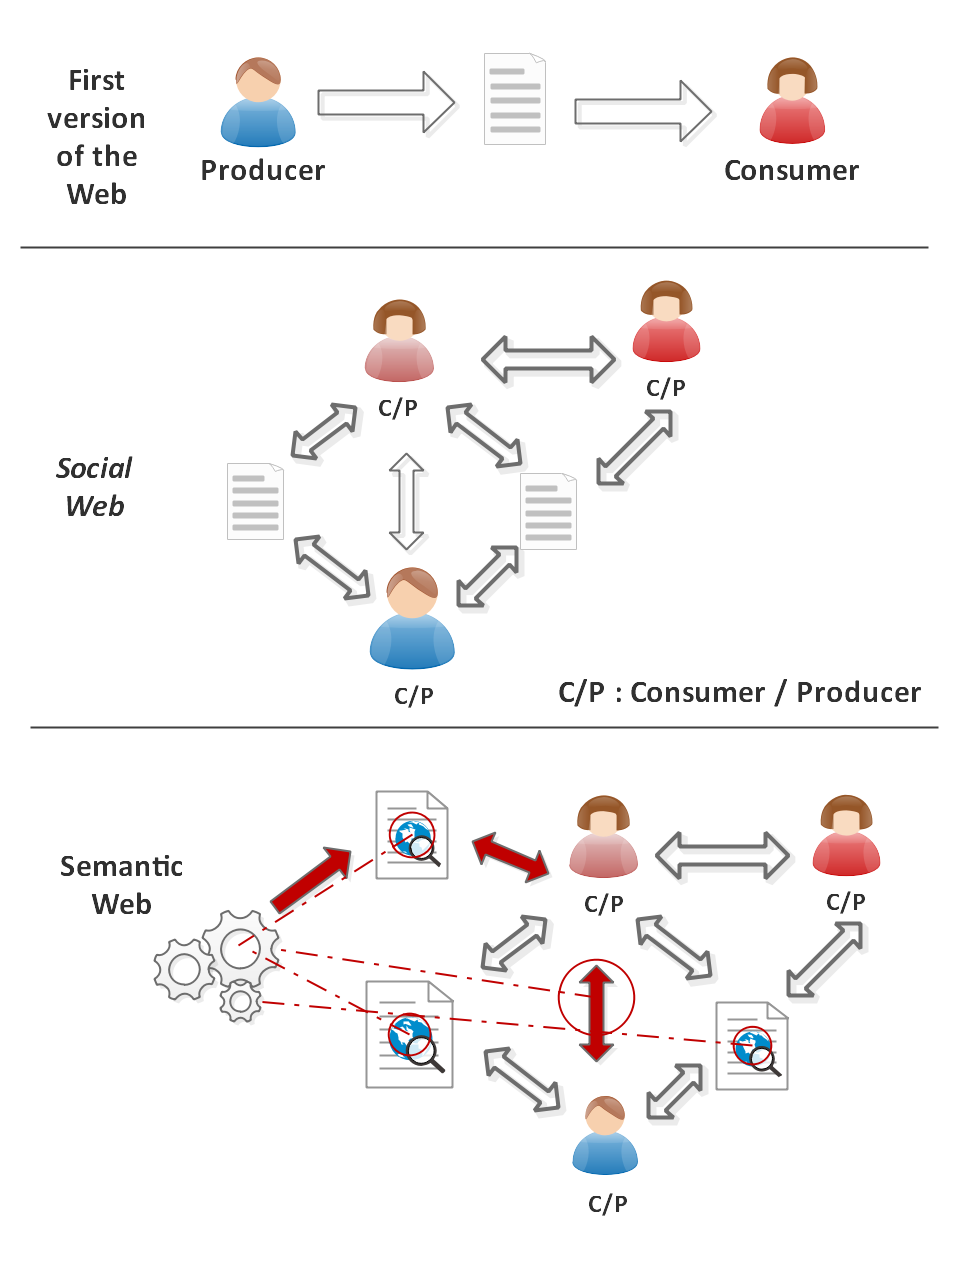
\includegraphics[scale=0.4]{peeps}
\caption{The evolution of Web}
\label{comparison}
\end{figure}



\begin{table}[H]
\centering
\caption{Web's versions comparison}
\label{comparisontab}
\begin{tabular}{|c|c|c|}
\hline
\rowcolor[HTML]{C0C0C0} 
First version of the Web        & Social Web            & Semantic Web    \\ \hline    
Dictated       & Socially constructed & Contextualy reinvented \\ \hline
Read-only      & Wildly read-write    & Portable and Personal                          \\ \hline
Company focus  & Community focus      & Individual focus                               \\ \hline
Home pages     & Blogs / Wikis        & Lifestreams / Waves                            \\ \hline

Web forms      & Web applications     & Smart applications                             \\ \hline
Owning content & Sharing content      & Consolidating content                          \\ \hline
HTML / Portals & XML/ RSS /DOM ...   & RDF /RDFS/ OWL ...                     \\ \hline
\end{tabular}
\end{table}


 
\section{Semantic Web architecture}
The architecture of semantic Web, as suggested by Tim Berners-Lee in 2000, \cite{archi} is shown in the figure \ref{fig_arch} below.  


\begin{figure}[H]
\centering
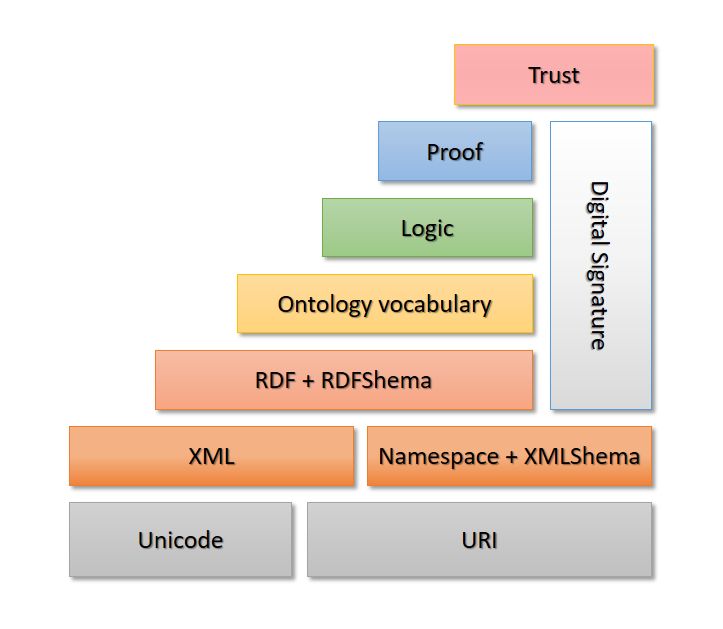
\includegraphics[scale=0.6]{arch11}
\caption{First semantic Web architecture}
\label{fig_arch}
\end{figure}


\begin{itemize}
\item The first layer is composed by URIs to give unique identifiers and Unicodes that provides every character a unique number no matter what the statform is. It allows data to be transported through many different systems without corruption.

\item In the next layer, XML allows the transportation of data between statforms, and Namespace that gives objects a referred name.

\item RDF and RDFS layers are the bases and the fundamentals of semantic Web. They describe taxonomies of concepts and properties. RDF is a simste assertions language used for describing resources in the World Wide Web. It is designed to represent information in the form of triples, such as subject, predicate and object.  

\item RDFS extends RDF vocabulary to allow describing taxonomies of classes and properties. Classes (generalized categories) and properties (predicates or binary relations) can be arranged into hierarchies. In addition, it extends definitions for some of the elements of RDF.

\item Ontologies make the collaboration between human and computers easier by sharing not only the syntax but also the semantic of Web resources.

\item The Logic layer is used to develop an advanced reasoning capabilities for knowledge extraction and efficient decision making.

\item The Proof layer defines a rule-based inference system which allows to derive assertions from known assertions described in RDF, OWL, etc.

\item Finally, the trust layer, which is based on the two previews layers (Logic and Proof), controls and determines the veracity of the information and the trust of the source of data.
\end{itemize}




%%kappa 

In 2005, W3C has suggested a new way to present the  architecture of semantic Web as we see in the figure  \ref{fig_archnew} . What is new with this architecture that is the Ontology layer is divided in two alternatives ,OWL (Ontology Web Language) a standard language to describe ontologies and Rules which is a base-rules language.

The new architecture shown in the figure \ref{fig_archnew} above is the current semantic Web standard and is subtle to change in the future.

\begin{figure}[H]
\centering
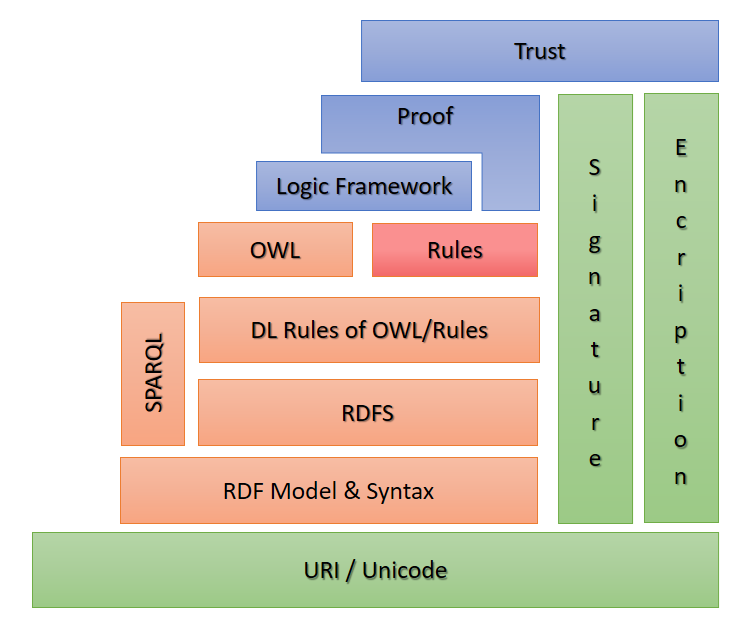
\includegraphics[scale=0.6]{arch21}
\caption{Current semantic Web architecture}
\label{fig_archnew}
\end{figure}





\section{Semantic Web Languages and technologies}
With the creation of Semantic Web, many languages were developed, most of them are based on XML or use it as a syntax. However, XML don't provide the semantic of resources, that is why other languages are used to specify the meaning of data.

\subsection{RDF}
RDF (Resource Description Framework) is a standard model for data interchange on the Web. RDF has features that facilitate data merging even if the underlying schema differ, and it specifically supports the evolution of schema over time without requiring all the data consumers to be changed.
Based on triples, RDF extends the linking structure of the Web to use URIs to name the relationship between subjects and objects. Using this simple model, it allows structured and semi-structured data to be mixed, exposed, and shared across different applications. This linking structure forms a directed, labeled graph, where the edges represent the named link between two resources, represented by the graph nodes. This graph view is the easiest possible mental model for RDF and is often used in easy-to-understand visual explanations.
Since RDF is using XML and it is at the base of the semantic Web, so that all the other languages corresponding to the upper layers are built on top of it.


RDF provides XML-based syntax, called RDF\slash XML. A piece of RDF\slash XML code written below :\\

\begin{lstlisting}[captionpos=b, caption=RDF Triple example, label={rdftriple},
basicstyle=\footnotesize,frame=single]
1. <?xml version="1.0"?>
2. <rdf:RDF xmlns:rdf="http://www.w3.org/1999/02/22-rdf-syntax-ns#"
3.          xmlns:isi="http://isi.tn#">

4.    <rdf:Description rdf:about="http://isi.tn#Student">
5.       <isi:hasName>"Safoine"</isi:hasName>
6.    </rdf:Description>

7. </rdf:RDF>       
\end{lstlisting}

\noindent Line numbers are added to the example which are explained down below:
\begin{itemize}
    \setlength{\itemsep}{0cm}
    \setlength{\parskip}{0cm}

    \item \textbf{Line 1}: contains standard XML declaration \texttt{<?xml version="1.0"?>}, which indicates that the content of that file is XML, and provides XML version which is used inside.	
    \item \textbf{Line 2}: starts from tag \texttt{rdf:RDF}, which indicates that the following XML content syntax is RDF. The \texttt{xmlns:rdf} defines a namespace identified by the URI \url{http://www.w3.org/1999/02/22-rdf-syntax-ns#}, and tells that all tags prefixed with \texttt{rdf:} are parts of the namespace. That namespace is used for terms from RDF vocabulary.
    \item \textbf{Line 3}: defines another prefix \texttt{isi:}, which represents namespace \url{http://www.isi.tn#}. URI \url{http://isi.tn#} is used for vocabulary terms defined by organization \texttt{isi.tn}.
    \item \textbf{Lines 4-6}: provide RDF/XML code, which describes the statement shown in  the graph \ref{fig_rdf}. 
    \item \textit{Line 4} begins from tag \texttt{rdf:Description} which indicates the start of description of a resource. Next, using attribute \texttt{rdf:about}, identifies the resource the statement is about (the subject of the statement), by providing its URI \url{http://isi.tn#Student}. 
    \item \textbf{Line 5}: declares property element \texttt{isi:hasName} for the subject resource, where both predicate and object of the statement are represented. The value of the property identified by namespace \url{http://isi.tn#hasName} is a stain literal \texttt{Safoine}. 
    \item \textbf{Line 6}: closes \texttt{rdf:Description} element.
    \item \textbf{Line 7}: indicates the end of \texttt{rdf:RDF} element.
\end{itemize}

\subsubsection{RDF vocabulary}
\noindent RDF vocabulary \cite{rdfv} is a defined set of predicates that can be used in an application.
The vocabulary defined by the RDF specification is indicated below:\begin{itemize}
\item \texttt{<rdf:RDF>}: Is the root element of an RDF document. It defines the XML document to be an RDF document. It also contains a reference to the RDF namespace:
\item \texttt{<rdf:Description>}: Contains elements that describe the resource.
\item \texttt{<rdf:Bag>}: Is used to describe a list of values that do not have to be in a specific order, it may contain duplicate values.
\item \texttt{<rdf:Seq>}: Is used to describe an ordered list of values.
\item \texttt{<rdf:Alt>}:is used to describe a list of alternative values (the user can select only one of the values).
\end{itemize}
Vocabulary is used as a backbone for RDF Schema, where that limited vocabulary is extended.



\subsubsection{RDF Graph}
RDF is a data model presented by a graph. The structure of every RDF model is presented by triples, each one is composed by a subject, a predicate and an object. A set of those triples forms a graph as it shown in the figure below  \ref{fig_rdf}:
\begin{itemize} 
\item Subject: The resource to describe.
\item Predicate: A property asserted to the resource.
\item Object: Is data or a other resource, it's the value of the property in the predicate.
RDF graph has at least two nodes and a property to relate them. Some of those nodes are represented by an ellipse referring to an entity with an URI ,other nodes are represented by a rectangle and having a literal value to express the entity directly.
 \end{itemize}
 \begin{figure}[H]
\centering
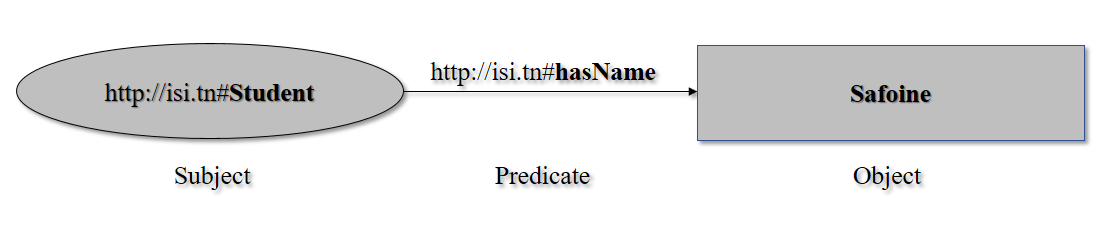
\includegraphics[scale=0.5]{rdf}
\caption{Example of RDF triple }
\label{fig_rdf}
\end{figure}


\subsubsection{Graph nodes types}
To describe Web resources, RDF graph nodes have two types: \begin{itemize}
\item URI: Is used to present resources described in RDF graph and to avoid designation confuse.
\item Literal:It describes property value and has two types: \begin{itemize}
\item Simple literal: It a string,presenting property value, it may have language attribute.
\item Typed literal: Presented by a string and an URI of that string type.
\end{itemize}
\item Empty: An empty node is an unique node that can be used in many triplets in the same RDF graph. 
\end{itemize}
RDF structure is an oriented and ordered graph based on triples. The subject of a triple may be  an URI or an empty node, the property is always presented by an URI and the object may be an URI, literal or an empty node. 

\subsubsection{RDF Graph's Relations}
An RDF triple is the description of a declaration, a logical expression or a claim in the world. RDF graph is the conjunction of triples. There are various relationships that can be established between graphs:\begin{itemize}
\item Involvement: An RDF graph A leads to an other RDF graph B, if every thing that make A true makes B also true. If A involved B, then the truth of A is proved or demonstrated then the truth of B is established.
\item Equivalence: Two RDF graphs A and B are equivalent if they describe the same information. A and B are equivalent if and only if A involved B and B involved B
\item Inconsistency: An RDF graph is inconsistent if it has an internal contradiction and there is no way that the description in the graph may be true.
\end{itemize}



\subsection{RDFS}
RDF Schema  \cite{RDFSchema} extends RDF vocabulary to allow describing taxonomies of classes and properties. Classes (generalized categories relations) and properties (predicates or binary relations) can be arranged into hierarchies. 
The RDF Schema provides a type system for RDF. The RDFS is technologically advanced compared to RDF since it provides a way to build an object model from which the actual data is referenced and which tells what things really mean. Briefly, the RDF Schema allows users to define resources with classes, properties, and values. The concept of RDF class is similar to the concept of class in object-oriented programming languages such as Java and C++. A class is a structure of similar things and inheritance is allowed (e.g: rdfs:subClassOf). This allows resources to be defined as instances of classes allowing classes to be organized in a hierarchical fashion. 
\newpage
\subsubsection{RDFS structure}
\label{sub:rdfsConstructs}

\noindent RDFS main structure and vocabulary is presented by:
\begin{itemize}
    \setlength{\itemsep}{0cm}
    \setlength{\parskip}{0cm}

\item \textbf{Classes}: Class tag are described in the table \ref{class_tag} below:
\begin{table}[H]
\centering
\caption{RDFS Class tags}
\label{class_tag}
\begin{tabular}{|l|l|}
\hline
rdfs:Resource  & All things described by RDF are resources, it is the class of everything \\ \hline
rdfs:Class     & Declares a resource as a class of another resource                       \\ \hline
rdfs:Literal   & Literal values, such as strings or integers                              \\ \hline
rdfs:Datatype  & It's a class of datatypes                                                \\ \hline
rdf:XMLLiteral & The class of XML literal values                                          \\ \hline
rdf:Property   & Class of properties                                                      \\ \hline
\end{tabular}
\end{table}

   %% \item \textbf{Classes}: \texttt{rdfs:Resource}: All things described by RDF are resources, it is the class of everything. \texttt{rdfs:Class}: Declares a resource as a class of another resource. \texttt{rdfs:Literal}: Literal values, such as strings or integers. \texttt{rdfs:Datatype}: It's a class of datatypes. \texttt{rdf:XMLLiteral}: The class of XML literal values. and \texttt{rdf:Property}: Class of properties. Example:
%%\textbf{Example}:
%%{\tt \small
%%\begin{verbatim}
%%<rdf:Description rdf:about="http://isi.tn#Student">
 %%  <rdf:type rdf:resource=Mehdi/>
%%</rdf:Description>
%%\end{verbatim}
%%}
%%
%%{\tt \small
%%\begin{verbatim}
%%<rdfs:Class rdf:ID="StudentID">
 %%  <rdfs:subClassOf rdf:resource="L3FSI01"/>
%%</rdf:Class>
%%\end{verbatim}
%%}

    \item \textbf{Properties}: Property tags are shown in table \ref{prop_tag} below:
    
\begin{table}[H]
\centering
\caption{RDFS Property's tags}
\label{prop_tag}
\begin{tabular}{|l|l|}
\hline
rdfs:domain        & Declares the class of the \texttt\{subject\} in a triple block   \\ \hline
rdfs:range         & Declares the class or datatype of the object in a triple block   \\ \hline
rdf:type           & Property used to state that a resource is an instance of a class \\ \hline
rdfs:subClassOf    & Allows to declare hierarchies of classes                         \\ \hline
rdfs:subPropertyOf & Allows to declare hierarchies of properties                      \\ \hline
rdfs:seeAlso       & Relates a resource to another with additional exstanation        \\ \hline
rdfs:isDefinedBy   & Relates a resource to its definition                             \\ \hline
rdfs:label         & Provides friendly name of resource                               \\ \hline
rdfs:comment       & Provides a human-readable description of a resource              \\ \hline
\end{tabular}
\end{table}
    
    %%\texttt{rdfs:domain}: Declares the class of the \texttt{subject} in a triple block. \texttt{rdfs:range}: Declares the class or datatype of the object in a triple block. \texttt{rdf:type}: Property used to state that a resource is an instance of a class. \texttt{rdfs:subClassOf}: Allows to declare hierarchies of classes. \texttt{rdfs:subPropertyOf} Allows to declare hierarchies of properties.\texttt{rdfs:seeAlso}: Relates a resource to another with additional exstanation.
     %% \texttt{rdfs:isDefinedBy}: Relates a resource to its definition.
     %%\texttt{rdfs:label}: Provides friendly name of resource.
      %%\texttt{rdfs:comment}: Provides a human-readable description of a resource).\\
     

%%{\tt \small
%%\begin{verbatim}
%%<rdf:Property rdf:ID="StudentID">
  %% <rdfs:subPropertyOf rdf:resource="isStudent"/>
   %%<rdfs:domain rdf:resource="Peoste"/>
   %%<rdfs:ranage rdf:resource="isiStudents"/>
%%</rdf:Property>
%%\end{verbatim}
%%}

      
\end{itemize}

%%\medskip

\noindent The fact is, that there is lack of any notion of negation or disjunction in RDFS. It provides only a very limited notion of existential quantification. This makes for RDFS language \textit{"very limited expressive power"}.

\subsection{Ontology}
The term ontology \cite{ontonew} derives from Greek, with “onto” meaning “being”, and “logos” usually interpreted as “science”; so that ontology, as traditionally understood, is the science or study of being.
Ontologies in computer science are conceptual schema that provides a logical description of data. An ontology defines terms which with to represent knowledge. For present purposes, one can think of data as that expressible in ground atomic facts and knowledge as that expressible in logical sentences with existentially and universally quantified variables. An ontology defines the vocabulary used to compose complex expressions such as those used to describe resource constraints in a stunning  problem. From a finite, well-defined vocabulary one can compose a large number of coherent sentences. That is one reason why vocabulary, rather than form, is the focus of specifications of ontological commitments. 

Ontologies are classified according to its subject and its structure, we recognize:\begin{itemize}  
\item \textbf{Domain ontologies}: This type of ontology is the most used in semantic Web applications, it describes resources of a specific domain and can be reuse in different applications in the same domain.

\item\textbf{Application ontologies}: It contains knowledge which are necessarily for a given application.
\item \textbf{Generic ontologies}: A high level ontology because it describes very generic resources like time, space, state, process,etc.
The concepts contained in an ontology of the domain are included in the concepts of a generic ontology.
\end{itemize} 
The conception of an ontology consider the fact that the semantic Web is distributed, that's why we can extend existing ontologies, or use them to create new ones .
To use terms in the ontology, we must indicate from what ontology it comes, that why we use prefixes that every ontology should  begin with in \textit{rdf:RDF} tag.
After that comes the content of the ontology putted in \textit{Owl:Ontology} tag.
The different component of an ontology are classes,properties and individuals.

\textbf{Classes}: A class in a group of individuals that have similar characteristics and may be classed hierarchically by a taxonomy.
All defined classes are children of a super-class called. \textit{OWL:Thing}. As the oriented object languages, inheritance is available in ontologies using the property \textit{subClassOf} of rdfs.

\textbf{Properties}: A property expresses a fact about a class and their individuals e.g the color of a car, it model and power are properties of car class.
There are two types of properties:\begin{itemize}
\item Properties allow to link individuals to other individuals.
\item Properties of data type allow to give a literal value to an individual.
\end{itemize}

\textbf{Individuals}: The definition of an individual is expressing a fact about a class, individuals are also called axioms and there are two types of them:\begin{itemize}
\item Fact that belongs to a class, indeed we declare an individual and its property's literal value.
\item Fact concerning individual's identity, we may face problems when axioms in a class are not unique and to solve that ambiguity we use properties like \textit{owl:sameAs},\\             \textit{owl:differentFrom} and \textit{owl:allDifferent}.
\end{itemize}

\subsection{OWL}
OWL (Ontology Web Language) \cite{OWL} is a W3C recommendation since 2004 . On top of RDF and RDFS, OWL comes with a larger vocabulary and stronger syntax, having a similar foundation as other Semantic Web languages, OWL has greater machine interpret ability. OWL provides a variety of constructors to express properties(roles), objects(individuals) and classes(concepts) as showed below:  \begin{itemize}
    \item Connectors of logical description (intersection, union, various restrictions..)
    \item Properties of defined classes
    \item Cardinality
    \item Types of properties
    \item Characteristics of properties (e.g. symmetry, transitivity)
\end{itemize}

The table \ref{tab:owlConstructors} \cite{HLP08} below presents different OWL constructors and their DL Syntax equivalent. 

\begin{table}[H]
\centering
\begin{tabular}{ |>{\tt}l|l|l| }
    \hline
    \multicolumn{1}{|c|}{\textbf{Constructor}}  & \multicolumn{1}{c|}{\textbf{DL Syntax}}   & \multicolumn{1}{c|}{\textbf{Example}} \\ \hline
    intersectionOf                              & $C_{1}\sqcap\cdots\sqcap C_{n}$           & $Human \sqcap Male$ \\ \hline
    unionOf                                     & $C_{1}\sqcup\cdots\sqcup C_{n}$           & $\mathit{Doctor} \sqcup \mathit{Lawyer}$ \\ \hline
    comstementOf                                & $\lnot C$                                 & $\lnot \mathit{Male}$ \\ \hline
    oneOf                                       & ${x_{1}\cdots x_{2}}$                     & ${\mathit{john},\mathit{mary}}$ \\ \hline
    allValuesFrom                               & $\forall P.C$                             & $\forall \mathit{hasChild}.\mathit{Doctor}$ \\ \hline
    someValuesFrom                              & $\exists r.C$                             & $\exists \mathit{hasChild}.\mathit{Lawyer}$ \\ \hline
    hasValue                                    & $\exists r.\{x\}$                         & $\exists \mathit{citizensOf}.\{\mathit{USA}\}$ \\ \hline
    minCardinality                              & $(\geq nr)$                               & $(\geq 2~\mathit{hasChild})$ \\ \hline
    maxCardinality                              & $(\leq nr)$                               & $(\leq 2~\mathit{hasChild})$ \\ \hline
    inverseOf                                   & $r^{-}$                                   & $\mathit{hasChild}^{-}$ \\ \hline
\end{tabular}
\caption{OWL constructors}
\label{tab:owlConstructors}
\end{table}

OWL is based on axioms, those axioms are used to make assertions,e.g assertions of relationships between classes or properties.
%%TABLEAU 

Furthermore, the table \ref{tab:owlAxioms} \cite{HLP08} below presents different axioms on the OWL syntax and their DL Syntax equivalent. 

\begin{table}[H]
\centering
\begin{tabular}{ |>{\tt}l|l|l| }
    \hline
    \multicolumn{1}{|c|}{\textbf{Axiom}}    & \multicolumn{1}{c|}{\textbf{DL Syntax}}   & \multicolumn{1}{c|}{\textbf{Example}} \\ \hline
    subClassOf                              & $C_{1} \sqsubseteq C_{2}$                 & $\mathit{Human} \sqsubseteq \mathit{Animal} \sqcap \mathit{Biped}$ \\ \hline
    equivalentClass                         & $C_{1} \equiv C_{2}$                      & $\mathit{Man} \equiv \mathit{Human} \sqcap \mathit{Male}$ \\ \hline
    subPropertyOf                           & $P_{1} \sqsubseteq P_{2}$                 & $\mathit{hasDaughter} \sqsubseteq \mathit{hasChild}$ \\ \hline
    equivalentProperty                      & $P_{1} \equiv P_{2}$                      & $\mathit{cost} \equiv \mathit{price}$ \\ \hline
    disjointWith                            & $C_{1} \sqsubseteq \lnot C_{2}$           & $\mathit{Male} \sqsubseteq \lnot \mathit{Female}$ \\ \hline
    sameAs                                  & ${x_{1}} \equiv {x_{2}}$                  & $\mathit{President\_Bush} \equiv \mathit{G\_W\_Bush}$ \\ \hline
    differentFrom                           & ${x_{1}} \sqsubseteq \lnot {x_{2}}$       & $\mathit{john} \sqsubseteq \lnot \mathit{peter}$ \\ \hline
\end{tabular}

\caption{OWL axioms}
\label{tab:owlAxioms}
\end{table}


Using DL syntax ,we are able create OWL equivalents by serializing them into XML as shown below :
\[
\mathit{Female} \sqcap \mathit{Male}
\]

{\tt \small
\begin{verbatim}
<owl:intersectionOf rdf:parseType="Collection">
   <rdf:Description rdf:about="#Female"/>
   <rdf:Description rdf:about="#Male"/>
</owl:intersectionOf>
\end{verbatim}
}

\[
\mathit{Student} \sqcup \mathit{Professor}
\]

{\tt \small
\begin{verbatim}
<owl:unionOf rdf:parseType="Collection">
   <rdf:Description rdf:about="#Student"/>
   <rdf:Description rdf:about="#Professor"/>
</owl:unionOf>
\end{verbatim}
}

\[
\exists \mathit{hasChild}.\mathit{Lawyer}
\]

{\tt \small
\begin{verbatim}
<owl:Restriction>
   <owl:onProperty rdf:resource="#hasChild"/>
   <owl:someValuesFrom rdf:resource="#Lawyer"/>
</owl:Restriction>
\end{verbatim}
}

\[
\exists \mathit{citizensOf}.\{\mathit{Tunisia}\}
\]

{\tt \small
\begin{verbatim}
<owl:Restriction>
   <owl:onProperty rdf:resource="#isCitizenOf"/>
   <owl:hasValue rdf:resource="#Tunisia"/>
</owl:Restriction>
\end{verbatim}
}

\bigskip

\subsubsection{OWL and reasoners}
One of reasons why OWL is based on DL is that we can use DL reasoning services in OWL based applications. The decidable ensures, that consistency of OWL DL ontology can be checked by DL reasoners. Reasoners can be also used to infer information from asserted facts.\\
The most popular reasoners in OWL community are :Pellet, FaCT, FaCT++, KAON2 or HermiT, RACER.
These reasoners provide reasoning services for tools that create and maintain ontologies like Protégé, Swoop, OilEd and TopBraid Composer.\\
The number of tools designed for OWL have increased , that motivate the community to develop ontologies for various fields like medicine, geology, biology, geography, astronomy, agriculture or defence, in which ontologies are adopted.

\subsubsection{OWL sublanguages}
There are three variants of OWL that W3C specification defines. These sublanguages are:OWL Lite, OWL DL and OWL Full that provides different level of expressiveness (increasingly in mentioned order) \cite{semwebp}. Each one of them is an extension of its predecessor. 
We have three sublanguages in OWL: \begin{itemize}
\item  \textbf{OWL Lite}: The simplest version, it support the classification hierarchies with simple constraints. It's not widely used  and acts as the entry point for Semantic Web application developers.
\item  \textbf{OWL DL}: Includes OWL Lite, it's the most used version of OWL. It was designed to provide maximum expressiveness possible while retaining computational decidable and automated reasoning.
\item  \textbf{OWL Full}: The most powerful OWL version in expressiveness. Includes OWL DL. Provides different semantic than predecessors.
\end{itemize}
\subsubsection{OWL 2}
OWL2 \cite{OWL2} has the same structure of OWL1 almost all of it components are present. OWL adds more functionality with respect to OWL1. Some of the new features are syntactic sugar while others offer new expressively, including:\begin{itemize}
\item Keys
\item Property chains
\item Richer data types, data ranges
\item Qualified carnality restrictions
\item Asymmetric, reflexive, and disjoint properties
\item Enhanced annotation capabilities 
\end{itemize}

OWL2 can be represented in a new format that is called the Manchester Syntax, its main objective is to ease the read/write process of DL Ontologies.\\
Also OWL2 has also its own sub-languages (profiles), we can mention:
\begin{itemize}
\item \textbf{OWL2 EL}: It is particularly suitable for applications where very large ontologies are needed. It enables polynomial time algorithms for all the standard reasoning tasks.
\item  \textbf{OWL2 QL}: Enables conjunctive queries to be answered in LogSpace using standard relational database technology; it is particularly suitable for applications where relatively lightweight ontologies are used to organize large numbers of individuals and where it is useful or necessary to access the data directly via relational queries(e.g. SQL).
\end{itemize}
\subsection{SPARQL}
SPARQL(SPARQL Protocol And RDF Query Language) \cite{SPARQL} is a W3C recommendation since January 2008 as a standard to query data in RDF graphs. A SPARQL query is a definition of a graph pattern through variables and constants. 

SPARQL has several query forms. These query forms use the solutions from pattern matching to form result sets or RDF graphs. 
For example, we will perform different SPARQL queries on the triple shown on the listing \ref{sparqltriple} below:

\begin{lstlisting}[captionpos=b, caption=Queried RDF triple, label={sparqltriple},
basicstyle=\footnotesize,frame=single]
// <http://exemple.isi/book/book1> <http://purl.org/dc/terms/title> "Learning C++"   
\end{lstlisting}

\begin{itemize}

\item \textbf{SELECT}: The query consists of two parts: the SELECT clause identifies the variables to appear in the query results, and the WHERE clause provides the basic graph pattern to match against the data graph.\\



QUERY:
{\tt \small
\begin{verbatim}
SELECT ?title
WHERE{
<http://example.isi.tn/book/book1> <http://purl.org/dc/terms/title> ?title.
}  
\end{verbatim}
}

RESULT: 
\bigskip
\begin{table}[H]
\centering
\caption{SPARQL query result}
\label{my-label}
\begin{tabular}{|c|}
\hline
?title         \\ \hline
"Learning C++" \\ \hline
\end{tabular}
\end{table}

\item \textbf{ASK}: Return true if the query match data in RDF, otherwise return false.\\
{\tt \small
\begin{verbatim}
@prefix foaf:       <http://xmlns.com/foaf/0.1/> .
:a  foaf:name       "Mehdi" .
:a  foaf:homepage   <http://work.example.isi.tn/Mehdi/> .
:b  foaf:name       "Safoine" .
:b  foaf:mbox       <mailto:safoine@example.isi.tn> .
\end{verbatim}
}
\newpage
QUERY: 
{\tt \small
\begin{verbatim}
PREFIX foaf:    <http://xmlns.com/foaf/0.1/>
ASK  { ?person foaf:name  "Mehdi". }
\end{verbatim}
}
RESULT: True.
\item \textbf{CONSTRUCT}: Returns an RDF graph by restricting the values in the data models.\\
QUERY:
{\tt \small
\begin{verbatim}
PREFIX foaf:    <http://xmlns.com/foaf/0.1/>
PREFIX vcard:   <http://www.w3.org/2001/vcard-rdf/3.0#>
CONSTRUCT   { <http://example.isi.tn/person#Mehdi> vcard:FN ?name }
WHERE   { ?x foaf:name ?name .}
\end{verbatim}
}
RESULT: 
{\tt \small
\begin{verbatim}
@prefix vcard: <http://www.w3.org/2001/vcard-rdf/3.0#>\\
<http://example.isi.tn/person#Mehdi> vcard:FN "Mehdi" .\\
\end{verbatim}
}
\item \textbf{DESCRIBE}: Returns a RDF graph who sets the corresponding resource.\\
\textbf QUERY:
{\tt \small
\begin{verbatim}
PREFIX foaf:   <http://xmlns.com/foaf/0.1/>
DESCRIBE ?x
WHERE    { ?x foaf:name "Mehdi". }
\end{verbatim}
}
\textbf{RESULT}:
{\tt \small
\begin{verbatim}
@prefix foaf:       <http://xmlns.com/foaf/0.1/> .
:a  foaf:name       "Mehdi" .
:a  foaf:homepage   <http://work.example.isi.tn/Mehdi/> .
\end{verbatim}
}
\end{itemize} 
\subsection{Annotation}
Semantic annotation is the process of attaching additional information to various concepts (e.g. people, things, places, organizations etc) in a given text or any other content. Unlike classic text annotations for reader’s reference, semantic annotations are used by machines to refer to.
When a document (or another piece of content, e.g. video) is semantically annotated it becomes a source of information that is easy to interpret, combine and reuse by our computers. Annotation can be manual, semi-automatic (based on automatic suggestions), or fully automatic. Manual annotation tools allow users to add annotations to web pages or other resources, and share these with others. An example annotation would relate the text “Paris” to ontology, identifying it as a city and as capital of "France". Automatic tools can perform similar annotations (such as named-entity recognition \cite{nlp}) without manual intervention. 

\section*{Conclusion}
The Semantic Web is not a dependant technology but an
extension of the old ones, in which the information is given a well-defined meaning, a better enabling computers and people to work in cooperation. The first steps in weaving the semantic Web into the structure of the existing Web are already and still under way. In the near future, these developments will usher in significant new functionality as machines become more intelligent and able to process and "understand" the data that they merely display at present. The Semantic Web will bring structure to the meaningful content of Web pages, creating an environment where software agents roaming from page to page can readily carry out sophisticated tasks for users. 


%%%%% Chapter three
\chapter{Proposed approach: Building a graphic for visualizing unstructured data}
\label{chap_dev}
	
\section*{Introduction}

Data visualization is the process of displaying data/information in graphical charts, figures and bars. It is used as means to deliver visual reporting to users for the performance, operations or general statistics of an application, network, hardware or virtually any IT asset. \\

Data visualization is typically achieved by extracting data from the underlying IT system. This data is generally in the form of numbers, statistics and overall activity. The data is processed using data visualization software and is displayed on the system's dashboard. It is generally done to assist IT administrators in getting quick, visual and easy-to-understand insight into the performance of the underlying system. Most IT performance monitoring applications use data visualization techniques to provide statistical insight of performance of the monitored system.
\newpage




\section{Unstructured data}
Unstructured data represents any data that does not have a recognizable structure. It is unorganized and raw and can be non-textual or textual. For example, email is a fine illustration of unstructured textual data. It includes time, date, recipient and sender details and subject, etc., but an email body remains unstructured. Unstructured data also may be identified as loosely structured data, wherein the data sources include a structure, but not all data in a data set follow the same structure.
Unstructured data refers to data that follows a form that is less ordered than items like spreadsheet pages, database tables or other linear or ordered data sets. In fact, the term "data set" is helpful because it is associated with data that is in neat, accessible arrays, without any extra content, and that is linked or tagged in a specific structure. \\

Other instances of unstructured textual data include Word documents, PowerPoint presentations, instant messages, collaboration software, documents, books, social media posts and medical records. Non-textual unstructured data is generally created in media, such as MP3 audio files, JPEG images and Flash video files, etc. \\

Unstructured data usually does not include a predefined data model, and it may not match well with relational tables. Unstructured data is usually text heavy. However, it may include numbers and dates, as well as facts. This leads to ambiguities that are difficult to identify using conventional software programs. \\


The storage of huge volumes of unstructured data generated within an enterprise, if poorly managed, may lead to higher expenses. Data in hard copy documents or in an electronic format must be scanned in order for a search application to parse out ideas, depending on words used in certain contexts. This is known as enterprise or semantic search. \\

In customer-centered businesses, the data found in an unstructured form may be examined to enhance relationship marketing and customer relationship management (CRM). As social media apps, such as Facebook and Twitter, go mainstream, unstructured data development is likely to outrun the progress of structured data.  \\

\section{Proposed approach}
In order to accomplish the On demand graphical representation, our approach has essentially 3 steps to follow: Document analysis, Ontology construction, Document Annotation as shown in the figure \ref{fig_app}. We will enumerate and specify each of these main steps.  
%%description gènérale de l'approche  avec figure



\begin{figure}[H]
\centering
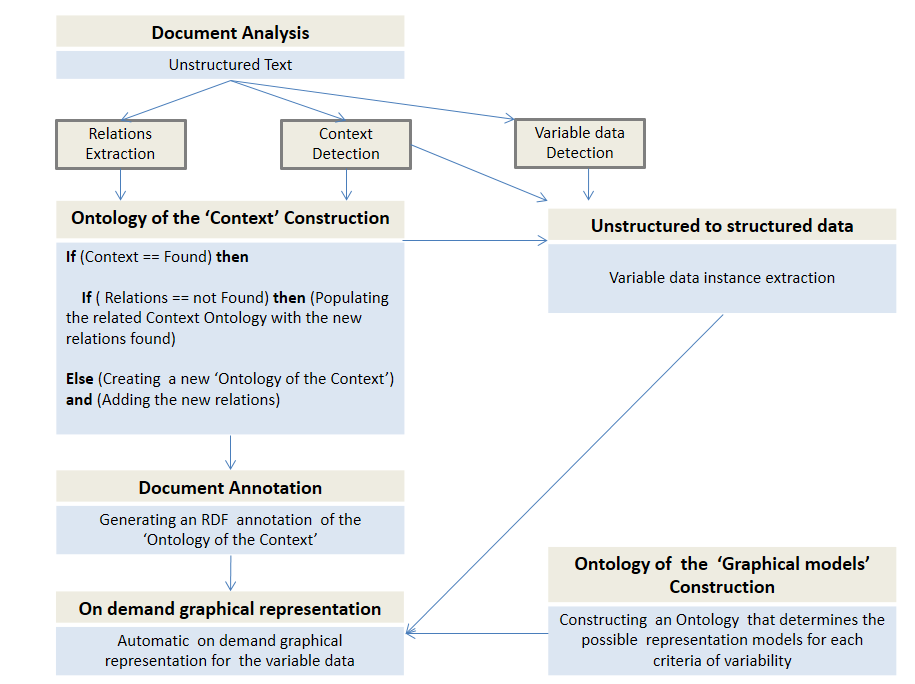
\includegraphics[scale=0.6]{plsfinal}
\caption{Execution flow of the on demand graphical representation}
\label{fig_app}
\end{figure}

\section{Document analysis}
\label{sec_anal}
%%Unstructured text analysis
Natural Language Processing (NLP) \cite{nlp} is a way for computers to analyze, understand, and derive meaning from human language in a smart and useful way. By utilizing NLP, developers can organize and structure knowledge to perform tasks such as automatic summarization, translation, named entity recognition, relationship extraction, sentiment analysis, speech recognition, and topic segmentation (see Figure \ref{fig_nlp}).

NLP is used to analyze text, allowing machines to understand how human’s speak. This human-computer interaction enables real-world applications like automatic text summarization, sentiment analysis, topic extraction, named entity recognition, parts-of-speech tagging, relationship extraction, stemming, and more. NLP is commonly used for text mining, machine translation, and automated question answering. 

NLP is characterized as a hard problem in computer science. Human language is rarely precise, or plainly spoken. To understand human language is to understand not only the words, but the concepts and how they’re linked together to create meaning. Despite language being one of the easiest things for humans to learn, the ambiguity of language is what makes natural language processing a difficult problem for computers to master. 

The figure \ref{fig_nlp} \cite{corenlp} below shows the overall system architecture of NLP.

\begin{figure}[H]
\centering
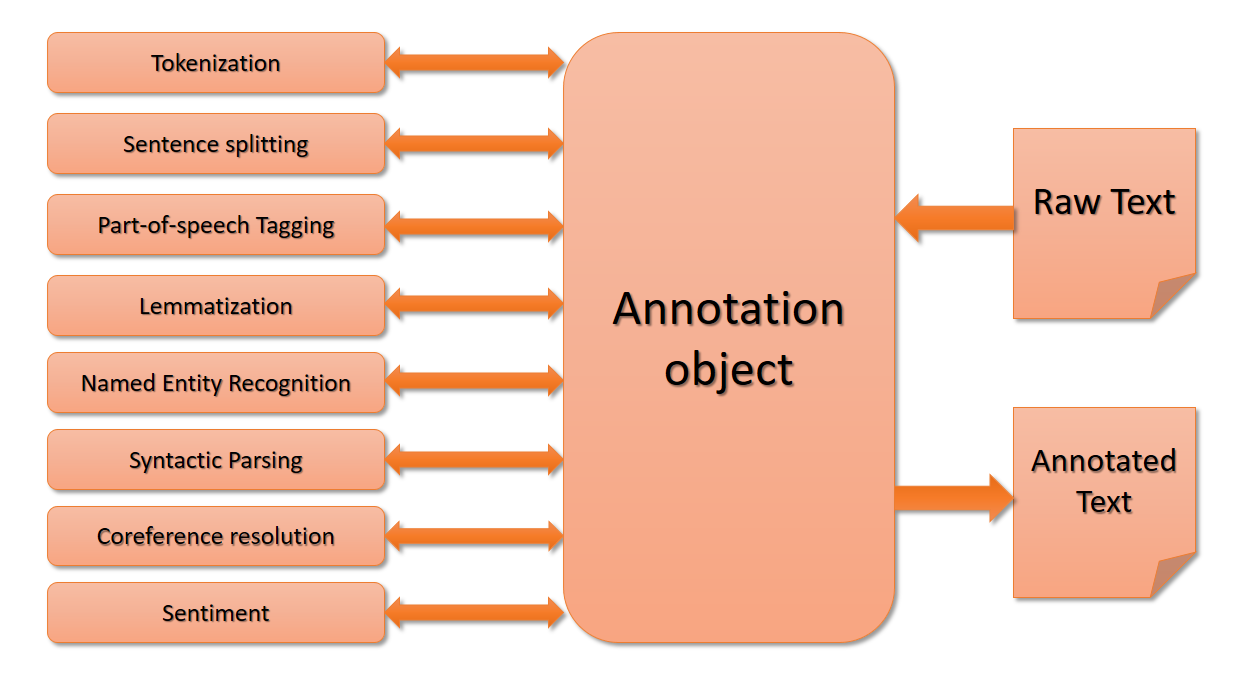
\includegraphics[scale=0.5]{nlpflow}
\caption{Overall system architecture of NLP}
\label{fig_nlp}
\end{figure}
\newpage

The process of analyzing a document can be categorized in four main steps: tagging, annotating, coreference and sentiment.

%%\renewcommand{\labelenumi}{\Roman{\enumiv}}
\begin{itemize}
   \item \textbf{Tagging\cite{corenlp}:} \\
   Tagging is a core task in Natural Language Processing. It consists in associating to each token a label providing certain information (e.g. syntactic category, number, verb tense…). Five main steps have been identified while tagging textual information: 
   \begin{itemize}
     \item \textbf{Sentences segmentation:} is the first step of the tagging process. A sentence can be defined as one or more words forming a syntactic unit. This segmentation allows dividing the text into its component sentences. 
     \item \textbf{Tokinization:} is the second step that allows identifying of the textual units that form the different sentences.
     \item \textbf{Tagging:} helps to classify words into their lexical categories and labeling them accordingly.
     \item \textbf{Lemmatization:} grants the representation of each word by its canonical form.
     \item \textbf{Syntactic parsing:} provides full syntactic analysis including through dependency representation between the words in order to identify the simple groups (nominal group, verbal group ...). 
   \end{itemize}
   \item \textbf{Named Entity Recognition:} \\
   Named Entity Recognition \cite{ner} labels sequences of words in a text which are the names of things, such as person and company names, or gene and protein names. It comes with well-engineered named entity recognizers for the English language. It particularly determines four classes (PERSON, ORGANIZATION, LOCATION, DATE).
   
   \item \textbf{Coreference resolution:} \\
   A Coreference is a relationship between two or more expressions in a text that refer to the same person or thing. The Coreference resolution \cite{corenlp} is the process in which we identify different reference chains. It is also known as Coreference in NLP techniques.
   
   \item \textbf{Sentiment:} \\
  Sentiment Analysis is the last method of NLP, it is a technique that is used to extract, identify, or otherwise characterize the sentiment content of a text unit. It is also known as "Opinion mining".

\end{itemize}

The first step in our proposed approach is analyzing an unstructured text document as an input data to detect the context related to that and to determine the variable data and statements using various NLP techniques \cite{maha}.   

We now present how to use these techniques to initially identify the context of a document, the named entities and the relations in-between them, and lastly, detecting the different variables that can be graphically plot. 



\subsection{Context detection}
\label{sec_21}

As the definition, a context is a part of a text or statement that surrounds a particular word or passage and determines its meaning. The context of a given document is identified from its main topics \cite{maha}. \\
The topics identification process can be acquired by obtaining the most important textual units. These units are keywords named "Key-terms candidates" which are usually different noun phrases.   \\
Some key-terms candidates are redundant in regard to the topic they represent. As a consequence, the similar key-terms candidates are grouped as a single entity named “class of subjects”. Then, the different subjects are classified according to their importance in the document. Finally, from each class of subjects, a single key-term that will represent all the others is selected. The different key-terms obtained represent the main topics of a document. The figure \ref{fig_topics} below shows the described process:

\bigskip

\begin{figure}[H]
\centering
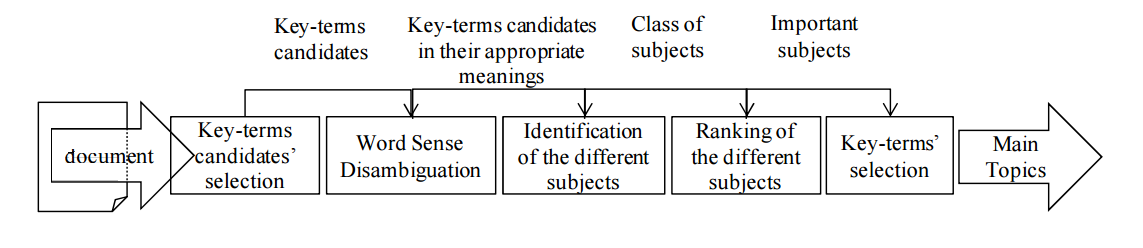
\includegraphics[scale=0.5]{topics}
\caption{The process of main topics identification }
\label{fig_topics}
\end{figure}

Among the topics found, we determine only one that will be representing the context of the document. The process of the context identification is described as follows: \\ 
We, first, calculate the similarity between all pairs of main topics by applying the similarity of Jiang and Conrath \cite{jiang}. The term which has the highest similarity rate with all the other identified main topics, is chosen as the most important topic of the document. \\

Once the most important topic of the document is identified, some additional information may be necessary. For instance, if we consider that the important topic is “Baccalaureate of 2017", the necessary additional information needed is the country where the academic qualification will be held. For example, the sentence “Tunisian Baccalaureate exams of 2017” represents a complex nominal group. In order to obtain the necessary additional information, we need to identify the different complex nominal groups in the document. A complex nominal group is a simple nominal group modified by one or two prepositional phrases.


\subsection{Extraction of significant variable data}
\label{extract_lab}
The process of extracting significant variable data \cite{maha} can be categorized in three main steps:
The first step employs the different named entities extracted in data processing stage in order to group the ones that belong to the same category (the names of persons, organizations, etc.) in a “class of category”. If we consider the following paragraph: 
“The French presidential election will be held on April 2017. The voters will go to the polls to pick their new president. Until now, the candidate, which has the highest scores of vote is Marine le Pen. This candidate credited with 27\%  of voting intention during the period of time 2-4 Mars, 2017. She obtained also 28\% during the period of time 14-16 Mars, 2017.”  
We can obtain four classes of category using the natural language processing techniques: “PERSON” that refer to a name of person, “DURATION” to a period of time, “DATE” to a given date and “PERCENT” to a percentage as shown in figure \ref{class_cat}.  

\begin{table}[H]
\centering
\caption{Different classes of categories}
\label{class_cat}
\begin{tabular}{|c|c|c|c|c|c|c|}
\cline{1-1} \cline{3-3} \cline{5-5} \cline{7-7}
\cellcolor[HTML]{FFFFFF}{\color[HTML]{333333} PERSON} &  & DURATION                                                                     &  & PERCENT                                             &  & DATE       \\ \cline{1-1} \cline{3-3} \cline{5-5} \cline{7-7} 
Marine le Pen                                         &  & \begin{tabular}[c]{@{}c@{}}14-16 Mars, 2017\\ 2-4 Mars, 2017\end{tabular} &  & \begin{tabular}[c]{@{}c@{}}27\%\\ 28\%\end{tabular} &  & April 2017 \\ \cline{1-1} \cline{3-3} \cline{5-5} \cline{7-7} 
\end{tabular}
\end{table}

Once the different classes of categories are extracted, the problem arises in entities of a same category that may belong to different concepts. Therefore, we need to gather the different named entities that belong to the same concept as a single entity called “class of concepts”. Considering the class of category “PERSON” that contains different names of candidates and voters as described in table \ref{class_of}.


\begin{table}[H]
\centering
\caption{Class of category}
\label{class_of}
\begin{tabular}{|c|}
\hline
Person                                                                                                   \\ \hline
\begin{tabular}[c]{@{}l@{}}Marine le Pen\\ François Fillon\\ Fabien Martin\\ Marcel Laurent\end{tabular} \\ \hline
\end{tabular}
\end{table}

In this case, the process must be able to differentiate between both concepts \textit{“candidate” and “voter”}. Using the \textif{“Ontology of the Context"}, we notice that \textit{“Marine Le Pen”} and \textit{“François Fillon”} belong to the concept \textit{“candidate”} while \textit{“Fabien Martin”} and \textif{“Marcel Laurent”} are unknown persons. Therefore, the classification will be based on belonging to the same concept and thus allowing us to obtain the following classes of concepts presented in table \ref{Different_class}.

\begin{table}[H]
\centering
\caption{Different classes of concepts}
\label{Different_class}
\begin{tabular}{|c|c|c|}
\cline{1-1} \cline{3-3}
Candidate                                                                &  & Unknown person                                                         \\ \cline{1-1} \cline{3-3} 
\begin{tabular}[c]{@{}l@{}}Marine le Pen \\ François Fillon\end{tabular} &  & \begin{tabular}[c]{@{}l@{}}Fabien Martin\\ Marcel Laurent\end{tabular} \\ \cline{1-1} \cline{3-3} 
\end{tabular}
\end{table}

After identifying the different classes of concepts, we move to the detection of variables step. Therefore, we need to identify the possible relationships between each couple of classes. To do this, some algorithms have been developed in  in order to extract the different variables and store them in a structured sheet format similar to the one presented in the. These algorithms aims to build a matrix M with n rows (representing the number of sentences of the document) and three columns representing respectively nouns, verbs and complements, that will be extracted from each sentence. Then, splits up the matrix M into several sub-matrices (Mk) based on synonyms verbs. Finally, identifies the variables that can be plot graphically.
The output of the extraction of variable data process after processing is the following table \ref{different_var}: 


\begin{table}[]
\centering
\caption{Different variables extracted}
\label{different_var}
\begin{tabular}{|c|c|c|}
\hline
Candidate                                                           & Duration                                                                  & Percent                                             \\ \hline
\begin{tabular}[c]{@{}c@{}}Marin le Pen\\ Marin le Pen\end{tabular} & \begin{tabular}[c]{@{}c@{}}2-4 Mars, 2017\\ 14-16 Mars, 2017\end{tabular} & \begin{tabular}[c]{@{}c@{}}27\%\\ 28\%\end{tabular} \\ \hline
\end{tabular}
\end{table}


\subsection{Relationship extraction}
\label{sec_22}

%%The process of automatic detection of variables will differentiate between categories of these variables and the different models of graphical representations. In this step, we need information concerning the graphical representation model and the variable data extracted from a given document. This process will be implemented using various NLP techniques.
Relation Extraction (RE) \cite{reeeeeeee} consists of the identification of the semantic relations between pairs of terms in unstructured or semi-structured natural language documents. Semantic relations are useful for several applications, including the acquisition of terminological data, construction and extension of lexical resources and ontologies, question answering, information retrieval, semantic web annotation, etc. In our proposed approach here, some existing text processing tools should be able to extract the relations between the variable data instances. The approach is consisted of mapping linguistic components with some syntactic relationship (a linguistic triple) and the mapping between terms and concepts is guided by a domain ontology and a named entity recognition system. A linguistic triple can contains three terms: A subject, a property and an object. E.g: A raw text containing the sentence "The lion belongs to the carnivores species." , the linguistic triple that should be extracted is: 
"lion" as the subject, "belong\_to" as the property and "carnivores" as the object. 



\section{Ontology Construction}

%%\section{Applied Ontologies}
\label{sec_3}
We use two ontologies in our proposed approach - the first one is the Ontology of the context generated after the detection of the the main topics, the context and the variable data, and secondly, the Graphical representation Ontology that is created manually. 
%%but in this step we will only focus on the automatic construction of the "Ontology of the context". 

\subsection{Ontology of the Context}
\label{sec_33}
Before jumping up and creating the context ontology, we must first look for other existing ontologies out there on the Internet using Ontology search engines like OntoSearch \cite{ontosearch}. If the context already exists, we will be using and populating it with our variable data and relations found retrieved from our analyzed document. And if the Ontology of the corresponding context is not found, we will proceed and create a new ontology related to the new context found.  
%%\begin{figure}[H]
%%\centering
%%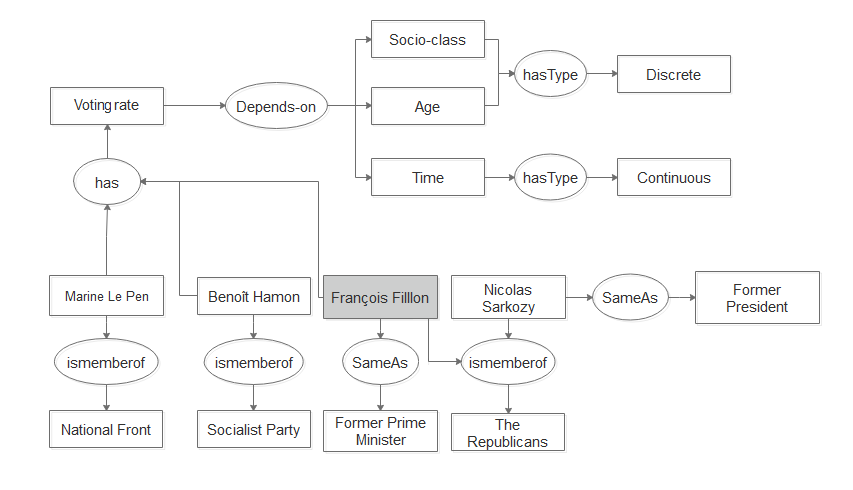
\includegraphics[scale=0.7]{contextOnt}
%%\caption{An example of a Context ontology}
%%\label{fig_context}
%%\end{figure}

\subsection{Ontology of the Graphical models}
\label{sec_44}
Generally, graphical models are those that were introduced by William Playfair where  he invented three of the four basic forms of graph: the statistical line graph, the bar graph and the pie graph. In 1786 he published “Commercial and Political Atlas” \cite{graphmodel} that contained 44 graphs. Modern statistical graphs are almost identical to those published by Playfair.

A Bar graph \cite{graphmodel} is drawn through columns of equal width and different heights. Three Types of Bar graphs are used to represent different data sets: The simple bar diagram, Compound bar diagram and Polybar diagram. The figure \ref{fig_bar} present a compound graph.

\begin{figure}[H]
\centering
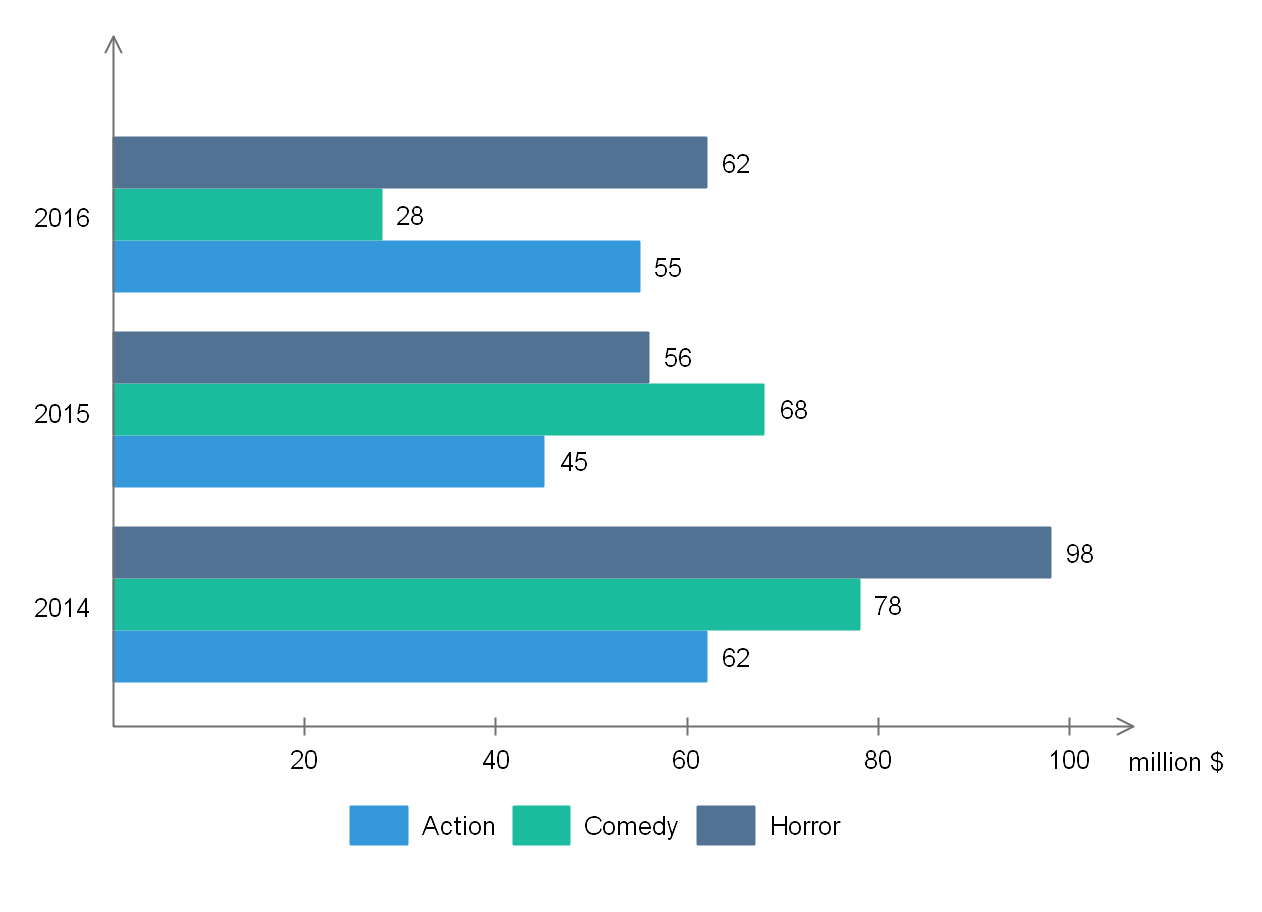
\includegraphics[scale=0.4]{compound}
\caption{Compound diagram of movie sales growth}
\label{fig_bar}
\end{figure}

A Pie diagram \cite{graphmodel} as presented in the figure \ref{fig_pie} is drawn to represent the total value of the given attribute using a circle. Dividing the circle into corresponding degrees of angle then represent the subsets of the data. Hence, it is also called as Divided Circle Diagram.


\begin{figure}[H]
\centering
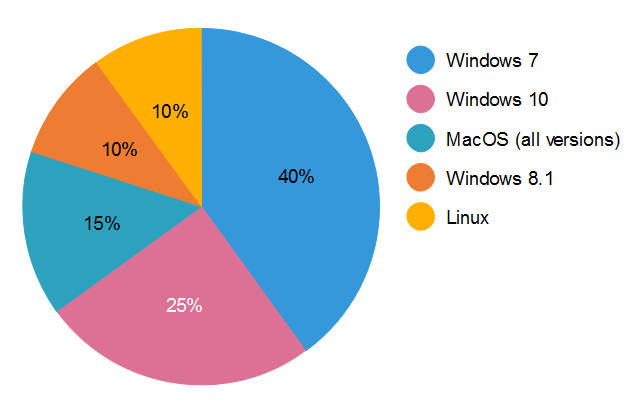
\includegraphics[scale=0.5]{piechart}
\caption{Pie diagram of operating systems usage}
\label{fig_pie}
\end{figure}
\newpage

The Line graphs \cite{graphmodel} as presented in the figure \ref{fig_poly} are usually drawn to represent the time series data. Example: temperature, rainfall, population growth, birth rates and the death rates, unemployment rates.

\begin{figure}[H]
\centering
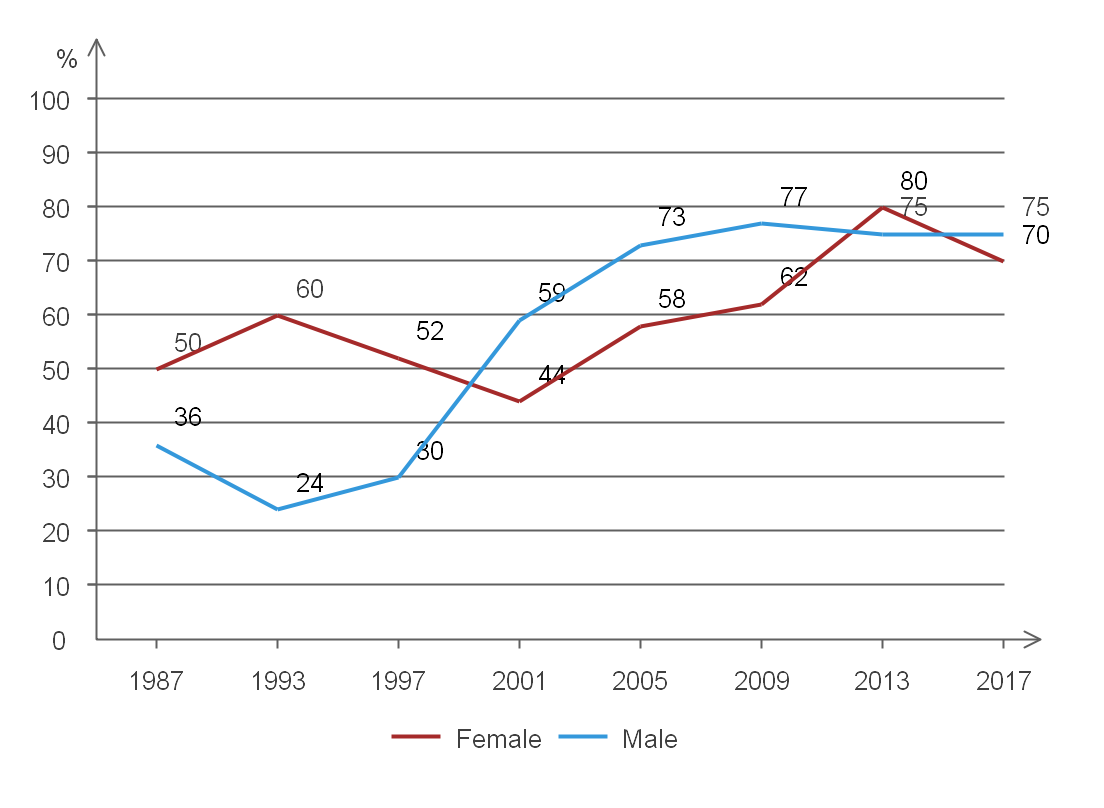
\includegraphics[scale=0.5]{linegraph}
\caption{Polygraph of unemployment rates}
\label{fig_poly}
\end{figure}


According to our proposed approach, we create a static and unique Ontology that is used each time the problem of the graphical representation on demand arises. The models are always the same whatever the data is about. Our idea is to refer to these models in the “Ontology of the Graphical Models” \cite{nour}.



\bigskip

\begin{figure}[H]
\centering
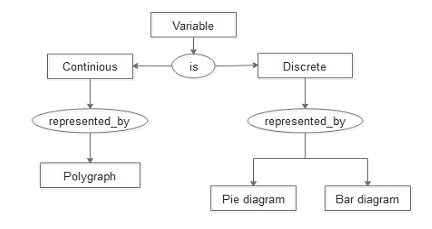
\includegraphics{Graphical_ontology}
\caption{Graphical models ontology }
\label{fig_Graphical_ontology}
\end{figure}


\section{Annotating the document}
\label{sec_55}

The primary purpose of annotating documents is to avoid reprocessing a document that has already been processed. A document can of course be processed several times in different contexts, but for a given context, it is a matter of "marking variable data", specifying which variable is considered as the “Principal Variable” and the others according to which this main variable varies. The annotation process is based on RDF and is deeply linked to the considered "Ontology of the Context". 




\section{On demand graphical representation}
\label{sec_66}

The on demand graphical representation relates to documents that have been already annotated. It is a fairly simple process that consists in applying the following steps:

\begin{enumerate}[label=(\alph*)]
\item Determining the variable to be represented in the y-axis. It is obtained from the overall context of the document. For example, if the context is "International Collegiate Programming Contest 2017" then the variable is the rate of solved problems. In this case the y-axis represents one or more teams for the contest.

\item  Determining the variable data to be represented in the x-axis. In our example ("International Collegiate Programming Contest 2017") can be measured according several criteria: time to represent its evolution, by duration, attempts , etc. \\
Each variable data has its own criteria which can be either discrete or continuous according to the Ontology of the "graphical models". This process of choosing criteria will be accomplished manually.
\item Retrieving the representation values from the extracted variable data instances of the current analyzed document, which guarantees that the graph is corresponding to the actual data of the context.
\item Granting the user the ability to select which graphical representation to be visualized regarding the obtained variable data and the criteria found by offering the ability to select which variable data to be shown in the x-axis and which available graphical representation to be visualized.
\end{enumerate}

 
\section*{Conclusion}


Semantic annotations describe the content of documents based on the concepts and relationships represented in an Ontology. In this context, Ontologies play an important role: they show the vocabulary and the knowledge of the field studied. These will be used to analyze the content of unstructured Web documents. The semantic annotation based on Ontology requires that it should be rich: it must represent not only the concepts and relations mentioned in the documents, but also the terms accompanied by their variants which in turn are used to denote these entities in the text.

\chapter{Experimentation and Implementation}
\label{chap_imp}

\section*{Introduction}

Semantic Web technologies have immense potential to transform the Internet into a distributed reasoning machine that will not only execute extremely precise searches, but will also have the ability to analyze the data it finds to create new knowledge. Our work uses the Semantic Web tools and infrastructure to show that these semantic technologies are sufficiently mature for expert use, and to solve some of the obstacles to Graphical Representation implementation. 

\section{Work environment}
\label{chap_work}

This section specifies and describes the hardware and software environment that we have used during the implementation of our work.  

\subsection{Hardware configuration}

We were using two computers where we deployed a local Web server in the first machine. The specifications of the computers are displayed in the next table \ref{tablehard}.
%%\caption{Hardware environment}
\begin{table}[H]
\centering
\caption{Hardware environment}
\begin{tabular}{|l|l|l|}
\hline
Specification & Lenovo G500 & Lenovo Z50 \\ 
\hline
RAM & 8GB & 8GB\\ 
\hline
Processor & Intel I3 3120M & Intel I7 4770U \\
\hline
Operating System & Windows 10 Pro & Windows 10 Pro \\ 
\hline
Screen Size & 15"6 & 15"6 \\ 
\hline
Type & Laptop & Laptop \\
\hline
\end{tabular}
\label{tablehard}
\end{table}

\subsection{Software environment }
\label{chap_soft}
In this section, we cite the different tools, languages, softwares and frameworks used in the development of this work.

%%\begin{wrapfigure}[4]{r}{2.5cm}
  %%   \vspace{-5mm}
%%    
\includegraphics[scale=0.2]{nlp}
%%\end{wrapfigure}
\textbf{- Standford CoreNLP} \cite{corenlp}
is a GPL-licensed framework of tools for processing English, Chinese, and Spanish. Includes tools for tokenization (splitting of text into words), part of speech tagging, grammar parsing (identifying things like noun and verb phrases), named entity recognition, and more.\\ 
The choice of the coreNLP over many other NLP tools (e.g: Apache openNLP, GATE, Natural Language Toolkit, etc.) consists to its performance, results and especially its variety of NLP techniques. \\ 

%%\begin{wrapfigure}[3]{r}{1.5cm}
%%     \vspace{-5mm}
%    
\includegraphics[scale=0.3]{owl}
%\end{wrapfigure}
\textbf{- OWL API} \cite{owlapi} is an open source Java API and reference implementation for creating, manipulating and serialising OWL Ontologies. It is now focused on the second version of the Web Ontology Language (OWL2).\\

%%\begin{wrapfigure}[3]{r}{2.5cm}
%%     \vspace{-5mm}
%%    
\includegraphics[width=2.5cm, height=2cm]{jena}
%%\end{wrapfigure}\textbf
{- Apache Jena}\cite{jena} is a Java framework for building Semantic Web applications. It provides a extensive Java libraries for helping developers develop code that handles RDF, RDFS, OWL and SPARQL in line with published W3C recommendations. \\

%\begin{wrapfigure}[3]{r}{2.5cm}
%     \vspace{-5mm}
%    
\includegraphics[width=2.5cm, height=2cm]{netbeans}
%%\end{wrapfigure}
\textbf{- NetBeans} is a powerful integrated development environment (IDE) that is used for developing Java desktop, mobile, and Web applications. It is free, open source, and has a large community of users and developers around the world. \\


%\begin{wrapfigure}[3]{r}{2.5cm}
%     \vspace{-5mm}
%%    
\includegraphics[width=2.5cm, height=2cm]{protetge}
%%\end{wrapfigure}
\textbf{- Protégé} is an Ontology building and editing software with full support of OWL2. It was developed by the Stanford Center for Biomedical Informatics Research at Stanford University, School of Medicine. It is built with JAVA and OWL API. It has desktop and Web version. \\

%\begin{wrapfigure}[3]{r}{2.5cm}
%     \vspace{-5mm}
%    
\includegraphics[width=2.5cm, height=1.2cm]{log4j}
%\end{wrapfigure}
\textbf{- Log4j:} Apache Log4j is a Java-based logging utility. It was originally written by  a Turkish engineer named Ceki Gülcü. It is now a project of the Apache Software Foundation.\\

\textbf{- Hermit:} is reasoner for Ontologies written using the Web Ontology Language (OWL). Given an OWL file, Hermit can determine whether or not the Ontology is consistent, identify subsumption relationships between classes, and much more. It is open-source and released under LGPL licence. 

The version (v1.3.8) of Hermit used with our +Context Ontology is fully compatible with OWLAPI 2.0.0. It is the reason why we had chosen that reasoner along our experimentation because Fact++ and Pellet reasoners were not compatible with the newest version of the OWLAPI and DL queries. \\

%\begin{wrapfigure}[3]{r}{2.5cm}
%     \vspace{-5mm}
%    
\includegraphics[width=2.5cm, height=2cm]{ajaxswing}
%\end{wrapfigure}
\textbf{- AjaxSwing:}  is a Web deployment platform for Java Swing applications. It allows Java desktop applications to run them as Web applications. It is available under commercial license that follows "something-for-something" philosophy, it has a free edition and its source code can be obtained under a small fee. \\

%\begin{wrapfigure}[3]{r}{2.5cm}
%     \vspace{-5mm}
%    
\includegraphics[width=2.5cm, height=2cm]{jsp}
%\end{wrapfigure}
\textbf{- Java Server Page (JSP):} is a text document that contains two types of text: static data, which can be expressed in any text-based format (such as HTML, SVG, and XML), and JSP elements, which construct dynamic content. \\

%\begin{wrapfigure}[3]{r}{2.5cm}
%     \vspace{-5mm}
%    
\includegraphics[width=2.5cm, height=2cm]{tomcat}
%\end{wrapfigure}
\textbf{- Apache Tomcat:} is an open source implementation of the Java Servlet, JavaServer Pages, Java Expression Language and Java WebSocket technologies. The Java Servlet, JavaServer Pages, Java Expression Language and Java WebSocket specifications are developed under the Java Community Process. \\

%\begin{wrapfigure}[3]{r}{2.5cm}
%     \vspace{-5mm}
%    
\includegraphics[width=2.5cm, height=2cm]{jquery}
%%\end{wrapfigure}
\textbf{- jQuery:} is a fast and lightweight JavaScript library. It presents many features including HTML/DOM manipulation, CSS manipulation, HTML event methods, AJAX, etc.

\section{Implementation}
\subsection{Document analysis}

During this step, we use several NLP techniques in order to extract the context and the relations from the document. Although, the process was a bit slow, we managed to determine the main context using Standford's CoreNLP and TextRank (a Java implementation of  the TextRank algorithm \cite{textmark}). The process is executed by extracting the topics (keywords) using CoreNLP by tokenizing the words in every sentence and lemmatizing these keywords. Later, we apply the tokens found into TextRank for more efficient topics extraction. Finally, we used WordNet \cite{wordnet} (a high efficient module that implements a variety of semantic similarity) in order to extract the context.\\

The next step comes in with the relations extraction that we have implemented using openIE \cite{openie} (Open information extraction) a Java implementation of an open IE (Information Extraction) system. This process is also conducted after text processing using NLP. An sample Java code is shown in the listing \ref{openieDefinition} below demonstrating the information extraction procedure.

\newpage

\begin{lstlisting}[captionpos=b, caption=Information extraction process definition in Java, label={openieDefinition},
basicstyle=\footnotesize,frame=single]
 //OpenIE
 Properties props = new Properties();

props.setProperty("annotators", "tokenize,ssplit,pos,lemma,depparse,natlog,openie");

StanfordCoreNLP pipeline = new StanfordCoreNLP(props);

 for (CoreMap sentence : doc.get(CoreAnnotations.SentencesAnnotation.class)) {
      // Get the OpenIE triples for the sentence
      Collection<RelationTriple> triples = sentence.get(NaturalLogicAnnotations.RelationTriplesAnnotation.class);
      // Printing  the triples 

    for (RelationTriple triple : triples ) {
        System.out.println(triple.confidence + "\t" +
            triple.subjectLemmaGloss() + "     \t" +
            triple.relationLemmaGloss() + "    \t" +
            triple.objectLemmaGloss());
    }        
\end{lstlisting}

Considering the context "The French presidential election of 2017" and the following sentence
"Emmanuel Macron is a candidate for the French presidential election 2017." The result of the Information extraction process is shown in the figure \ref{fig_ie} where it shows the minimal developed GUI (Graphical User Interface)  :

\newpage

\begin{figure}[htpb]
\centering
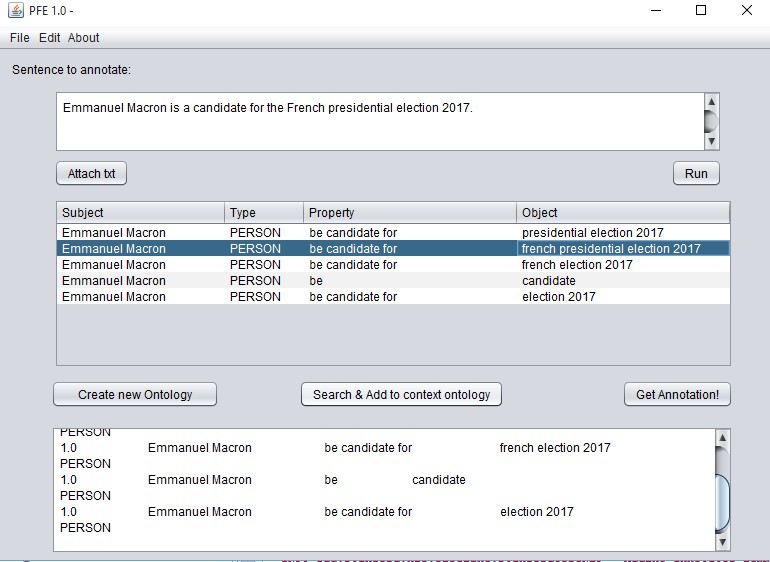
\includegraphics[scale=0.7]{exp1}
\caption{The process of main topics identification }
\label{fig_ie}
\end{figure}

\subsection{Ontology of the Context construction}

Once we have extracted the context and the relations from the desired document, we will construct the Ontology of the context.  \\
The first step is to allow the end user to choose which relations he desires to add to the ontology of the context since the information extraction process is not a very perfect tool so far, like we can see in The figure \ref{fig_const} below.
Once the user chooses the triple to be added to the Ontology of the Context, the application searches Ontologies for the extracted context . If we are able to find the right context, we will simply populate the Ontology that we have acquired during the search process. The population process in this step was implemented through the Hermit reasoner that helped with the search and the extraction of existing relations that we are going to add to the Ontology of the Context. A sample Java code shows how was the population of the context ontology was established is presented in the listing \ref{hermitt} below: \\

\begin{lstlisting}[captionpos=b, caption=Relations search using Hermit reasoner and a DL Query, label={hermitt},
basicstyle=\footnotesize,frame=single]
    public boolean HermitTest(String predicate,String object,OWLOntology ontology) throws ParserException {
    OWLReasoner reasoner = new Reasoner.ReasonerFactory().createReasoner(ontology);
        // Entities are named using IRIs. These are usually too long for use
        ShortFormProvider shortFormProvider = new SimpleShortFormProvider();
        // Create the DLQueryPrinter helper class. This will manage the
        // parsing of input and printing of results
        DLQueryEngine engine = new DLQueryEngine(reasoner, shortFormProvider);
        DLQueryPrinter dlQueryPrinter = new DLQueryPrinter(engine,shortFormProvider);
        // The DL query to search for the relations
        String query =  predicate+" some {"+object+"}";
        System.out.println(query);

        Set<OWLNamedIndividual> individuals = engine
                .getInstances(query, true);
        return dlQueryPrinter.getEntities("Properties", individuals);
    } 
\end{lstlisting}



Otherwise, if we are not able to find the appropriate domain of the Ontology of the context, we will construct a new one. We also gave the end user the opportunity to create a new ontology without looking for an existing Ontology of the context where it is shown in the figure \ref{fig_const}. This process was implemented using OWL API (v4.1.0).  

\begin{figure}[H]
\centering
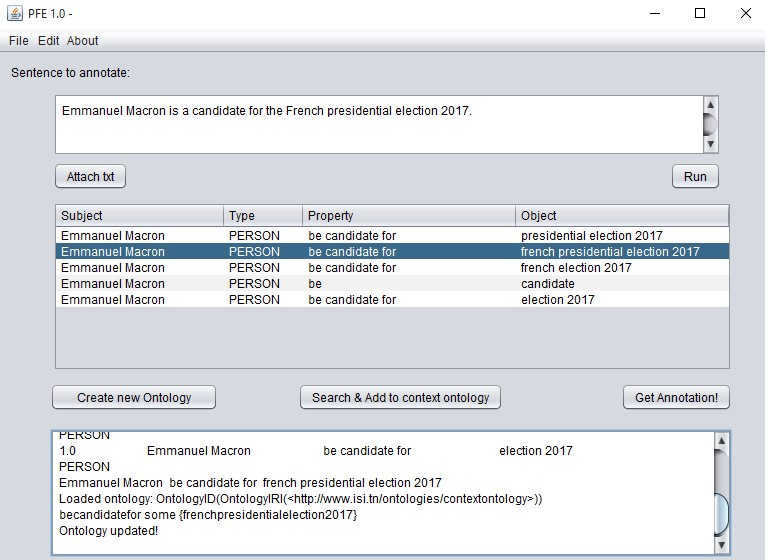
\includegraphics[scale=0.7]{exp2}
\caption{Constructing/populating the context ontology }
\label{fig_const}
\end{figure}
\bigskip

A sample Java code that shows how the population of the context Ontology was established is presented in the listing \ref{consteu} below: \\

\begin{lstlisting}[captionpos=b, caption=Context ontology population definition in Java, label={consteu},
basicstyle=\footnotesize,frame=single]
    //creating ontology manager
    OWLOntologyManager manager = OWLManager.createOWLOntologyManager(); 
    OWLOntology ontology;
            
    ontology = manager.loadOntologyFromOntologyDocument(contextOnt);

    //creating a new idividual from the relation found
    OWLIndividual individual = factory.getOWLNamedIndividual(IRI
            .create(ontologyIRI + "#"+sub.replaceAll("\\s","")));
            
    //matching the individual with the equivalent class    
    OWLClassAssertionAxiom classAssertion = factory.getOWLClassAssertionAxiom(clsAMethodA, individual);

    // validating the changes         
     manager.addAxiom(ontology, classAssertion);       
\end{lstlisting}


The Ontology will be generated in the OWL/XML format that is a bit easy to understand by humans. We chose this format because it is well-formed and structured. Here's a sample of the OWL file after adding the  relation triple into the Ontology of the context. \\


\begin{lstlisting}[captionpos=b, caption=Ontology of the context OWL/XML result, label={consteu},
basicstyle=\footnotesize,frame=none]
    <!-- http://www.isi.tn/ontologies/contextontology#be -->
    <owl:ObjectProperty rdf:about="http://www.isi.tn/ontologies/
    contextontology#be"/>   
    <!-- http://www.isi.tn/ontologies/contextontology#becandidatefor -->
    <owl:ObjectProperty rdf:about="http://www.isi.tn/ontologies/contextontology#becandidatefor"/>
<!-- http://www.isi.tn/ontologies/contextontology#EmmanuelMacron -->
    <owl:NamedIndividual rdf:about="http://www.isi.tn/ontologies/contextontology#EmmanuelMacron">
        <rdf:type rdf:resource="http://www.isi.tn/ontologies/contextontology#PERSON"/>
        <becandidatefor rdf:resource="http://www.isi.tn/
        ontologies/contextontology#frenchpresidentialelection2017"/>
    </owl:NamedIndividual>
    <!-- http://www.isi.tn/ontologies/
    contextontology#FrancoisFillon -->
    <owl:NamedIndividual rdf:about="http://www.isi.tn/ontologies/contextontology#FrancoisFillon">
        <rdf:type rdf:resource="http://www.isi.tn/ontologies/contextontology#PERSON"/>
        <be rdf:resource="http://www.isi.tn/ontologies/contextontology#candidate"/>
    </owl:NamedIndividual>     
\end{lstlisting}

The figure \ref{graphonto} shows the structure of the constructed ontology of the context after the Population process.

\begin{figure}[H]
\centering
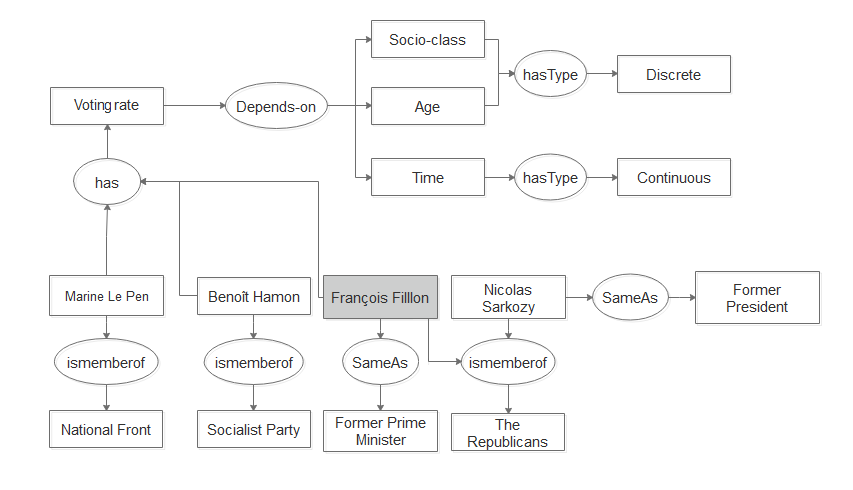
\includegraphics[scale=0.7]{contextOnt}
\caption{Ontology of the Context}
\label{graphonto}
\end{figure}

\subsection{Annotating the document}

The annotation process is the most important step for the on demand graphical representation. The annotation is generated by marking the principal variable and other variable data, accompanied with the relations that already existed in the Ontology of the context. This step is implemented throughout Apache Jena and OWL API in order to extract the different relations from the context ontology.\\ 
This sample java code shows the followed annotation generation process in the listing \ref{annot} below:


\begin{lstlisting}[captionpos=b, caption=Annotation generation definition in Java, label={annot},
basicstyle=\footnotesize,frame=single]
//gathering the individuals from the context ontology
Set<OWLNamedIndividual> inds=ontology.getIndividualsInSignature();
 \\getting the property values from the ontology
for (OWLNamedIndividual ind: inds){
if (!ind.getObjectPropertyValues(ontology).isEmpty()) {
System.out.println(ind.toStringID());

//combining the properties and the subjects found  together.
Map<OWLObjectPropertyExpression, Set<OWLIndividual>> map = ind.getObjectPropertyValues(ontology);
for (Map.Entry<OWLObjectPropertyExpression, Set<OWLIndividual>> entry : map.entrySet())
{
String subject = entry.getKey().toString().replaceAll(ontologyIRI.toString()+"#","");

//Creating an RDF property (Predicate)
Property propAnnot = ResourceFactory.createProperty(entry.getKey().toString());
//creating RDF model of the data found
Resource model1 = RDFmodel.createResource(ind.toStringID().replaceAll("\\s",""))
.addProperty(propAnnot,entry.getValue().toString());
}     
\end{lstlisting}
A sample of the generated RDF/XML annotation is shown in the listing \ref{notaaaa} below:

\begin{lstlisting}[captionpos=b, caption=RDF sample of the generated Annotation, label={notaaaa},
basicstyle=\footnotesize,frame=single]
<rdf:RDF
    xmlns:rdf="http://www.w3.org/1999/02/22-rdf-syntax-ns#"
    xmlns:dc="http://purl.org/dc/elements/1.1/"
    xmlns:graph="http://www.isi.tn/ontologies/contextontology#">
  <rdf:Description rdf:about="http://www.isi.tn/ontologies/contextontology#EmmanuelMacron">
    <graph:becandidatefor>France presidential election 2017</graph:becandidatefor>
  </rdf:Description>
  <rdf:Description rdf:about="http://www.isi.tn/ontologies/contextontology#FrancoisFillon">
    <graph:be>presidential nominee</graph:be>
  </rdf:Description>
  <rdf:Description rdf:about="http://www.isi.tn/ontologies/contextontology#Author">
    <dc:creator>Safoine Benhmida</dc:creator>
  </rdf:Description>
</rdf:RDF>    
\end{lstlisting}

\subsection{Constructing the ontology of graphical models}

As we have mentioned in the previous chapter that the Ontology of graphical models is static, we have constructed it manually using Protégé. A variable as shown in figure \ref{graph} may be continuous or discrete and each type has several graphical representation models. 

\begin{figure}[H]
\centering
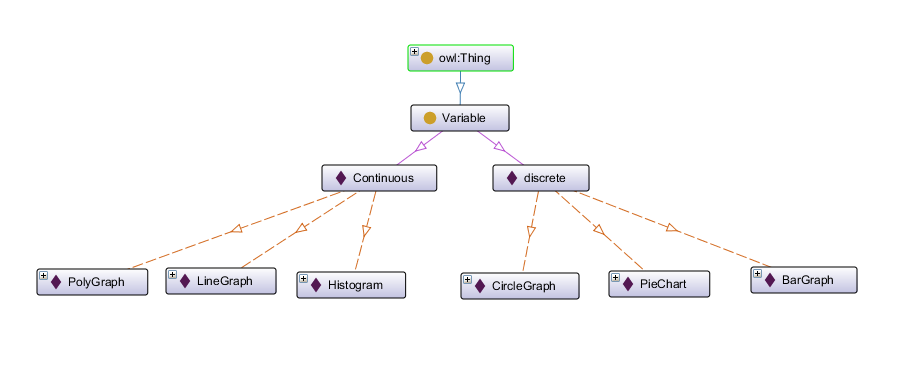
\includegraphics[scale=0.7]{onto}
\caption{Ontology of graphical models structure in Protégé}
\label{graph}
\end{figure}

\subsection{The on demand graphical representation}
The first step of implementing this model is to deploy a Web server that communicates with our based Java application. Thus, the process might seem difficult, we chose to use Apache Tomcat Web server since it is powerful and easy to deploy and most importantly, it is Java implemented. The figure \ref{tomcat} below show's the deployment process of the Web server using JavaSwing.  

\begin{figure}[H]
\centering
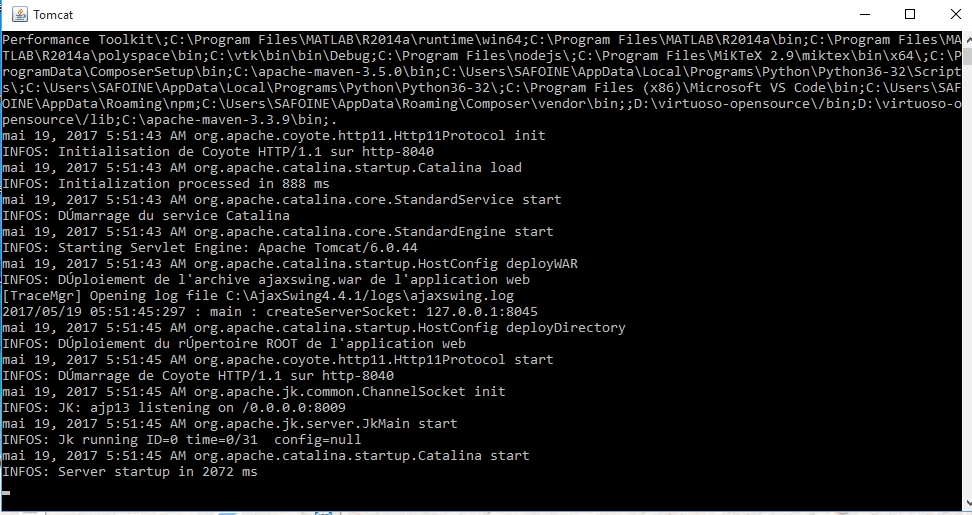
\includegraphics[scale=0.6]{tomcatserver}
\caption{Deploying the Apache Tomcat server}
\label{tomcat}
\end{figure}

During this process, the end user will be able to visualize any variable data that is related to the previously annotated Ontology of the context. Considering the data table  \ref{datatable} associated to the context "Presidential election United States 2016".   
\begin{table}[H]
\centering
\caption{Variable data table}
\label{datatable}
\begin{tabular}{|c|c|c|}
\hline
           & Hilary Clinton & Donald Trump \\ \hline
California & 40\%           & 60\%         \\ \hline
Texas      & 33\%           & 67\%         \\ \hline
New York   & 73\%           & 23\%         \\ \hline
Alabama    & 25\%           & 75\%         \\ \hline
\end{tabular}
\end{table}

The Y-axis element will be also automatically assigned as the principal variable. The variable data in the table will be assigned as a possible X-axis elements. After the analysis of the table is finished, the end user will be able to choose which variable data to visualize according to the available charts that are determined from the variable data criteria and the Ontology of the graphical models. The figure\ref{bargraph} shows the result of a "on demand graphical representation" of the data table \ref{datatable}: 

\begin{figure}[H]
\centering
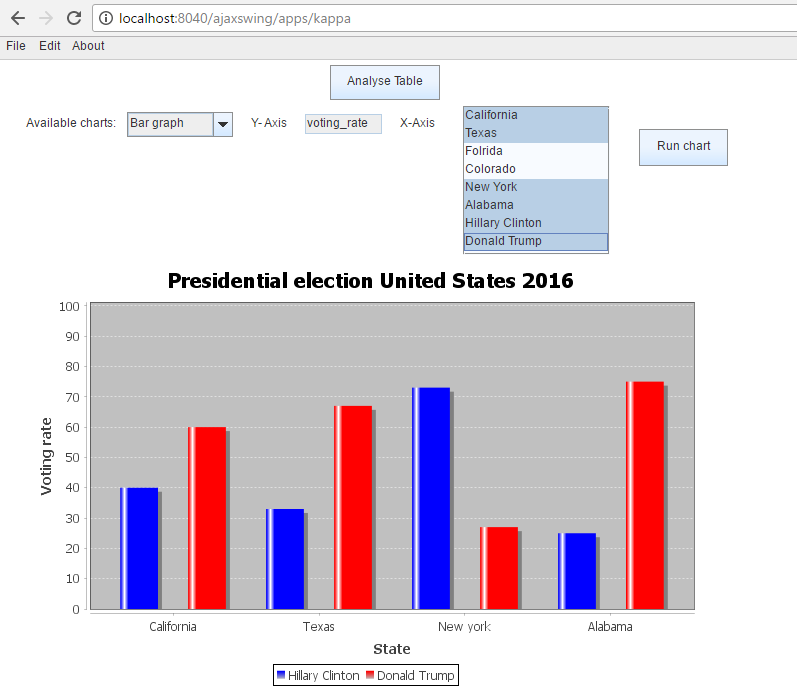
\includegraphics[scale=0.7]{chart1}
\caption{On demand bar graph }
\label{bargraph}
\end{figure}

The figure \ref{bargraph2} below show a result of graphical representation of variable data related to the context "The French presidential election of 2017".

\begin{figure}[H]
\centering
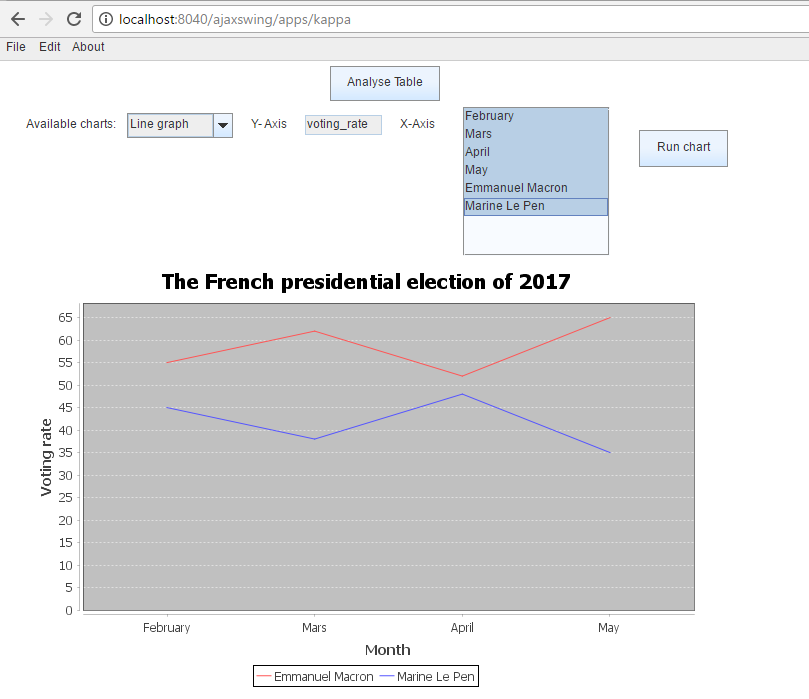
\includegraphics[scale=0.7]{chart2}
\caption{On demand line graph }
\label{bargraph2}
\end{figure}

\section{Conclusion}

Graphic representation is another way of analyzing numerical data. A graph is a sort of chart through which statistical data are represented in the form of lines or curves drawn across the coordinated points plotted on its surface. Graphs enable us in studying the cause and effect relationship between two variables. It helps with measuring the extent of change in one variable when another variable changes by a certain amount. Graphics also enable us in studying both time series and frequency distribution as they give clear account and precise picture of problem. Graphs are also easy to understand and eye catching.

\afterpage{\blankpage}

%%%%% To add new chapter, you should first add a chap_xx.tex file to the folder and add the following line
% \input{chap_xx}

%%%%% Conclusion
\addcontentsline{toc}{chapter}{General conclusion}
\chapter*{General conclusion}
\addcontentsline{toc}{section}{Summary of the main contributions}
\section*{Summary of the main contributions}

The main function of W3C is to standardize the representation and exchange of information on the Web. This objective should help to make information comprehensible to automated processes and users. New standards have been developed to allow the semantic representation of information in the form of languages derived from XML. This evolution is called Semantic Web. \\

Many languages have been developed within the framework of the semantic Web and most of these languages are based on the XML language. The OWL language and the RDF language are very important languages of the semantic Web. The OWL language allows to represent the ontologies, and it proposes to the machines a great capacity of execution of the Web content. The RDF is the first W3C standard for Web resource enrichment with detailed descriptions. These languages are used to represent the semantics associated with information, whatever its form and structure in the form of graphs. \\

Unstructured data is data that does not follow a specified format for big data. If 20 percent of the data available to enterprises is structured data, the other 80 percent is unstructured. Unstructured data is really most of the data that you will encounter. Until recently, however, the technology didn’t really support doing much with it except storing it or analyzing it manually. \\


The main contribution of this work is to implement an "On demand graphical representation" of unstructured documents on the Web. Another contribution of this work is to develop a tool that analyze unstructured text documents on the Web and extract context and all its relations. The process of the most important phases of our work can be summarized in five steps: 
 \begin{itemize}
    \item \textbf{The analysis of document} :To determinate the context and relations.
    \item \textbf{The construction of an ontology}:The creation or not of an ontology depend of the context of the analyzed document.
    \item \textbf{The annotation of the document} :Generating an RDF annotation of the context ontology.
    \item \textbf{Constructing the graphical models} : Constructing an ontology that determines the possible representation models for each criteria of variability.
    \item \textbf{The data visualization} :Automatic on demand graphical representation of the variable data.
    
    \end{itemize}
\addcontentsline{toc}{section}{Perspectives}    
    \section*{Perspectives}
We have managed to implement our proposed approach, Although we had lots difficulties since there wasn't enough tools and technologies that we can use in order to ease up the implementation phase. Thus, we had to develop our own algorithms and frameworks which was a a bit hard process to begin with.
For the moment our work isn't perfect, since the text analysis isn't very effective which led us to remodel the ontology population into a semi-automatic procedure and indeed, the analysis process concerns only a single document for the moment. Our future research concerns the graphic representation of data collected from multiple documents, and improving the text analysis process.


%\appendix


\backmatter


%%%%% Bibliography, in BibTeX format (the references.bib file)
\bibliographystyle{plain}
\bibliography{references}

%%\afterpage{\blankpage}

%\bibliographystyleA{plain}
%\bibliographyA{references}  

\afterpage{\blankpage}

\end{document}
